\documentclass[11pt,a4paper]{article}

% ==============================================================================
% PACKAGES AND ENCODING
% ==============================================================================
\usepackage[utf8]{inputenc}
\usepackage[T1]{fontenc}
\usepackage{lmodern}
\usepackage{amsmath,amssymb,amsfonts,amsthm,mathtools}
\usepackage{geometry}
\geometry{top=2.8cm,bottom=2.8cm,left=2.5cm,right=2.5cm}
\usepackage{booktabs,tabularx,multirow,array}
\usepackage{graphicx}
\graphicspath{{figures/}}
\usepackage{xcolor}
\definecolor{navyblue}{RGB}{0,51,102}
\definecolor{darkred}{RGB}{139,0,0}
\usepackage{hyperref}
\hypersetup{
    colorlinks=true,
    linkcolor=navyblue,
    citecolor=navyblue,
    urlcolor=navyblue,
    pdftitle={Kerr Geodesic Integrator: Technical Report},
    pdfauthor={Soumitra Pharikal}
}
\usepackage{cite}
\usepackage{cleveref}
\usepackage{microtype}
\usepackage{enumitem}
\usepackage{physics}
\usepackage{caption}
\captionsetup{font=small,labelfont=bf,width=0.92\linewidth}

% Numbering depth
\numberwithin{equation}{section}
\numberwithin{figure}{section}
\numberwithin{table}{section}

% ==============================================================================
% AUTHOR METADATA PLACEHOLDERS
% Edit these placeholders before final dissemination or repository archival
% ==============================================================================
\newcommand{\ReportAuthorName}{Soumitra Pharikal}
\newcommand{\ReportAuthorEmail}{24123@iiserbpr.ac.in}
\newcommand{\ReportAuthorAffiliation}{Indian Institute of Science Education and Research Berhampur (IISER Berhampur), India}
\newcommand{\ProjectRepositoryURL}{\url{https://github.com/SoumitraPharikal/kerr-geodesic-integrator}}

% ==============================================================================
% DOCUMENT METADATA
% ==============================================================================
\title{
    \vspace{-1.5cm}
    \textbf{\Large Numerical Integration, Constraint Preservation, and Celestial Shadow Construction in Kerr Spacetime} \\[0.5em]
    \large A Rigorous Computational Framework for Relativistic Geodesic Dynamics
}

\author{
    \textbf{\ReportAuthorName} \\
    \texttt{\ReportAuthorEmail} \\[0.3em]
    \small \ReportAuthorAffiliation
}

\date{\today}

% ==============================================================================
% MAIN DOCUMENT BODY
% ==============================================================================
\begin{document}

\maketitle

\begin{abstract}
We present the theoretical formulation, architectural design, and numerical verification of the \textsc{Kerr Geodesic Integrator}, an open-source computational physics package for null and timelike geodesic propagation in Kerr and Schwarzschild spacetimes. Formulated in eight-dimensional canonical Hamiltonian phase space in Boyer--Lindquist coordinates with analytical inverse-metric derivatives, the integrator employs an adaptive Dormand--Prince 8(5,3) Runge--Kutta solver with continuous polynomial dense output and event root-finding. We establish phase-space constraint preservation ($|2\mathcal{H}| \le 10^{-12}$) and analyze conserved quantities along geodesics. Benchmarks span the Schwarzschild photon sphere at $r=3M$, timelike circular orbits at the innermost stable circular orbit ($r_{\rm ISCO} = 6M$), Kerr equatorial circular photon orbits ($r_{\rm ph}^\pm$), epicyclic oscillations, and critical capture separatrices with logarithmic affine dwell divergence. Furthermore, we construct celestial Bardeen black-hole shadow boundaries across spins ($0 \le |a| \le M$) and inclinations, resolving the Near-Horizon Extreme Kerr (NHEK) line segment at supercritical inclinations ($\theta_o > \theta_{\rm crit} \approx 47.06^\circ$). In the near-polar limit ($\theta_o \ll 1$), we verify first-order speed dipole structure and curvature invariance, analyze the global polygonal chord deficit, and evaluate numerical convergence across 4,412 automated regression tests.
\end{abstract}

\vspace{0.5cm}
\noindent\textbf{Keywords:} General Relativity, Kerr Spacetime, Geodesic Integration, Hamiltonian Dynamics, Carter Constant, Black Hole Shadow, Near-Horizon Extreme Kerr, Numerical Astrophysics.

\clearpage
\tableofcontents
\clearpage

% ------------------------------------------------------------------------------
% MODULAR CHAPTER INCLUSIONS
% ------------------------------------------------------------------------------
\section{Introduction and Scientific Motivation}
\label{sec:introduction}

\subsection{Astrophysical Context and Conceptual Foundations}
The observational confirmation of black holes in general relativity represents one of the foundational triumphs of modern physics. Following the direct imaging of the supermassive black holes in the galaxy Messier 87 ($\text{M87}^*$) \cite{EHT2019_PaperI} and at the center of the Milky Way, Sagittarius A* ($\text{Sgr A}^*$) \cite{EHT2022_PaperI}, by the Event Horizon Telescope (EHT) Collaboration, relativistic ray-tracing and geometric shadow reconstruction have evolved from abstract theoretical gedankenexperiments into indispensable empirical tools for probing strong-field gravitation.

In general relativity, an uncharged, stationary, axisymmetric rotating black hole in vacuum is uniquely described by the Kerr metric \cite{Kerr1963}, parameterized entirely by its gravitational mass $M$ and spin angular momentum per unit mass $a \equiv J/M$. A black hole's event horizon marks a causal one-way membrane from which no signals or particles can escape to asymptotic infinity. Surrounding the horizon of a rotating black hole is the ergosphere, a region where spacetime frame-dragging is so intense that no physical observer can remain stationary relative to infinity.

Freely falling test particles and light rays traverse the curved spacetime along \textit{geodesics}---the four-dimensional curved-spacetime generalization of straight lines. A geodesic path $x^\mu(\lambda)$ parameterized by an affine parameter $\lambda$ satisfies the geodesic equation:
\begin{equation}
    \frac{d^2 x^\mu}{d\lambda^2} + \Gamma^\mu_{\alpha\beta} \frac{dx^\alpha}{d\lambda} \frac{dx^\beta}{d\lambda} = 0,
    \label{eq:geodesic_standard}
\end{equation}
where $\Gamma^\mu_{\alpha\beta}$ are the Christoffel connections. The magnitude of the four-velocity $u^\mu = dx^\mu/d\lambda$ defines the invariant dispersion relation:
\begin{equation}
    g_{\mu\nu} \frac{dx^\mu}{d\lambda} \frac{dx^\nu}{d\lambda} = -\mu^2,
    \label{eq:dispersion_intro}
\end{equation}
where $\mu = 0$ corresponds to massless particles (photons tracing null geodesics along the light cone) and $\mu > 0$ corresponds to massive particles (timelike geodesics, typically normalized such that $\mu = 1$ and $\lambda$ represents proper time per unit rest mass).

\subsection{Symmetries, Conserved Quantities, and the Role of Numerical Integration}
As established by Carter \cite{Carter1968}, geodesic motion in Kerr spacetime possesses a hidden dynamical symmetry: the presence of a non-trivial fourth constant of the motion, the Carter constant $\mathcal{Q}$, whose underlying irreducible second-rank Killing tensor $K_{\mu\nu}$ was subsequently identified by Walker and Penrose \cite{WalkerPenrose1970}. Together with the particle rest mass $\mu$, the conserved energy $E = -p_t$ (associated with stationarity via the timelike Killing vector $\partial_t$), and the axial angular momentum $L_z = p_\phi$ (associated with axisymmetry via the rotational Killing vector $\partial_\phi$), Carter's invariant decouples the Hamilton--Jacobi equation, rendering Kerr geodesic equations formally integrable in terms of elliptic integrals \cite{Chandrasekhar1983,Bardeen1973}.

Despite this formal mathematical integrability, direct numerical integration of the geodesic differential equations remains essential for scientific research:
\begin{enumerate}[label=(\roman*)]
    \item \textbf{Astrophysical Complexity:} Real black-hole environments involve magnetohydrodynamic accretion disks, radiative transfer, non-integrable spacetime perturbations, and structured emitting media \cite{Falcke2000,Luminet1979,CunninghamBardeen1973,Chael2021}, where analytical expressions cannot capture local interactions.
    \item \textbf{Camera-Plane Ray Tracing:} Generating synthetic black-hole images requires backward ray-tracing millions of null rays from pixel grids on a distant observer's camera to their emission origins, demanding efficient step-by-step numerical propagation.
    \item \textbf{Numerical Robustness:} Evaluating incomplete elliptic integrals and Jacobian elliptic functions across radial and polar turning points can encounter loss of significance and coordinate branch-cut ambiguities that direct numerical ODE integration avoids.
\end{enumerate}

\subsection{Hamiltonian Formulation and Methodological Distinctions}
Rather than integrating the second-order geodesic equations \eqref{eq:geodesic_standard} directly via Christoffel symbols, this framework adopts a canonical Hamiltonian formulation in eight-dimensional phase space $(x^\mu, p_\mu)$. The canonical Hamiltonian:
\begin{equation}
    \mathcal{H}(x^\mu, p_\mu) = \frac{1}{2} g^{\mu\nu}(x) p_\mu p_\nu
    \label{eq:hamiltonian_intro}
\end{equation}
yields a system of first-order Hamilton equations. This formulation offers significant computational advantages:
\begin{itemize}
    \item \textbf{Direct Momentum Conservation:} Metric symmetries manifest algebraically: because $\partial_t g^{\mu\nu} = 0$ and $\partial_\phi g^{\mu\nu} = 0$, the canonical equations $\dot{p}_t = -\partial\mathcal{H}/\partial t = 0$ and $\dot{p}_\phi = -\partial\mathcal{H}/\partial\phi = 0$ guarantee that $E$ and $L_z$ are preserved automatically up to floating-point round-off.
    \item \textbf{Elimination of Christoffel Symbols:} Equations of motion require only the analytical derivatives of the inverse metric components $\partial_i g^{\mu\nu}$, bypassing the 40 distinct connection coefficients of the Kerr metric.
    \item \textbf{Continuous Constraint Monitoring:} The value of $2\mathcal{H}$ serves as an independent, continuous monitor of numerical drift away from the null ($2\mathcal{H} = 0$) or timelike ($2\mathcal{H} = -1$) constraint surface.
\end{itemize}

\paragraph{Numerical Method Clarification:} We emphasize that the numerical solver implemented in this project is an \textit{adaptive explicit Runge--Kutta} method of Dormand--Prince 8(5,3) type (DOP853) equipped with continuous polynomial dense output, rather than a geometric \textit{symplectic} integrator. Standard explicit Runge--Kutta schemes are not symplectic. Instead of relying on symplectic geometry to bound phase-space volume, our framework achieves high-precision Hamiltonian constraint preservation ($|2\mathcal{H}| \le 10^{-12}$) through eighth-order local truncation error control, scale-invariant step-size adaptation, and active monitoring of the normalized Hamiltonian residual.

\subsection{The Black Hole Shadow and Celestial Bardeen Coordinates}
A prominent astrophysical observable modeled in this work is the black-hole shadow. When a black hole is illuminated by background or surrounding emission, photons that pass sufficiently close to the horizon are captured, creating a central region of darkness on the observer's sky bounded by a sharp silhouette \cite{Bardeen1973,Falcke2000,PerlickTsupko2022}. The boundary of this shadow corresponds to the critical trajectories that asymptotically separate capture from scattering to infinity, delineated in phase space by unstable spherical photon orbits at constant Boyer--Lindquist radius.

To describe the shadow quantitatively, an asymptotic observer situated at polar inclination $\theta_o$ projects the incoming null rays onto an imaginary celestial screen perpendicular to the line of sight. Following Bardeen \cite{Bardeen1973}, this plane is parameterized by Cartesian impact coordinates $(\alpha, \beta)$:
\begin{itemize}
    \item $\alpha$ represents the horizontal displacement perpendicular to the projected black-hole spin axis, measuring the impact parameter associated with frame-dragging and axial angular momentum ($L_z$).
    \item $\beta$ represents the vertical displacement parallel to the projected spin axis, measuring the impact parameter associated with latitudinal motion and Carter's constant ($\mathcal{Q}$).
\end{itemize}

\subsection{Project Scope and Document Organization}
This report documents the \textsc{Kerr Geodesic Integrator}, a Python-based computational framework developed to address these relativistic challenges. Specifically, the project investigates:
\begin{enumerate}[label=(\roman*)]
    \item Scale-invariant canonical phase-space propagation with adaptive step-size selection and sub-epsilon event root-finding (horizon cutoff, turning points, spatial escape).
    \item Independent dual-representation monitoring of Carter's constant ($\mathcal{Q}_{\rm polar}$ vs. $\mathcal{Q}_{\rm radial}$).
    \item Physical validation against known relativistic benchmarks: Schwarzschild photon spheres, circular orbits at the innermost stable circular orbit (ISCO), epicyclic frequencies, and critical photon scattering dwell times.
    \item Celestial Bardeen shadow boundary construction across spins $0 \le |a| \le M$ and inclinations $0 \le \theta_o \le \pi$, including the Near-Horizon Extreme Kerr (NHEK) vertical segment and exact-polar circular boundaries.
    \item Near-polar asymptotic perturbation expansions, proving the first-order invariance of shadow perimeter and curvature functionals.
    \item Rigorous convergence analysis of discrete polygonal boundary approximations against continuum references.
\end{enumerate}

The remainder of this paper is structured as follows: \Cref{sec:kerr_spacetime} presents the Boyer--Lindquist geometry and exact metric derivatives. \Cref{sec:hamiltonian_dynamics} develops the canonical Hamiltonian formulation and Carter invariants. \Cref{sec:numerical_architecture} details the integration architecture and dense-output event localization. \Cref{sec:conserved_quantities} establishes the scale-invariant conservation diagnostics. \Cref{sec:schwarzschild_validation,sec:kerr_physical_orbits,sec:photon_scattering} present the benchmark validation suite. \Cref{sec:shadow_construction,sec:extremal_nhek_and_polar,sec:near_polar_asymptotics} formulate shadow boundaries, NHEK structure, and near-polar expansions. \Cref{sec:numerical_error_analysis} provides the numerical convergence and error analysis. Finally, \Cref{sec:results_discussion,sec:limitations_future_work,sec:conclusions} discuss astrophysical implications, limitations, and concluding remarks.

\section{Kerr Spacetime and Mathematical Preliminaries}
\label{sec:kerr_spacetime}

\subsection{Coordinate Conventions and Line Element}
We adopt standard relativistic geometrized units where the speed of light and the gravitational constant are set to unity:
\begin{equation}
    c = G = 1.
\end{equation}
In this system, spacetime coordinates and black hole mass $M$ carry dimensions of length $[L]$, while the spin parameter $a \equiv J/M$ carries dimensions of length $[L]$ with the dimensionless spin parameter defined as $\chi \equiv a/M \in [-1, 1]$. We adopt the metric signature convention $(-, +, +, +)$ throughout.

In standard Boyer--Lindquist coordinates \cite{BoyerLindquist1967,MisnerThorneWheeler1973} ordered as $x^\mu = (x^0, x^1, x^2, x^3) = (t, r, \theta, \phi)$, with $t \in (-\infty, \infty)$, $r \in (0, \infty)$, $\theta \in [0, \pi]$, and $\phi \in [0, 2\pi)$, the Kerr metric line element is:
\begin{align}
    ds^2 &= -\left(1 - \frac{2Mr}{\Sigma}\right) dt^2 - \frac{4Mar\sin^2\theta}{\Sigma} dt\,d\phi \nonumber \\
    &\quad + \frac{\Sigma}{\Delta} dr^2 + \Sigma\,d\theta^2 + \left(r^2 + a^2 + \frac{2Ma^2r\sin^2\theta}{\Sigma}\right)\sin^2\theta\,d\phi^2,
    \label{eq:kerr_line_element}
\end{align}
where the fundamental auxiliary functions are defined by:
\begin{align}
    \Sigma(r, \theta) &\equiv r^2 + a^2\cos^2\theta, \label{eq:def_sigma} \\
    \Delta(r) &\equiv r^2 - 2Mr + a^2. \label{eq:def_delta}
\end{align}

\subsection{Horizons and Ergosphere Boundaries}
The roots of the radial metric function $\Delta(r) = 0$ define the geometric horizons of the black hole:
\begin{equation}
    r_\pm = M \pm \sqrt{M^2 - a^2}.
    \label{eq:horizon_radii}
\end{equation}
For subextremal black holes ($|a| < M$), $r_+$ represents the outer event horizon (a null hypersurface acting as an absolute causal one-way membrane), while $r_-$ represents the inner Cauchy horizon. In the extremal limit $|a| = M$, the two horizons coalesce into a single degenerate horizon at $r_+ = r_- = M$.

The boundary of the ergosphere corresponds to the static limit surface where the asymptotic timelike Killing vector field $\xi_{(t)} = \partial_t$ becomes null ($g_{tt} = 0$):
\begin{equation}
    r_{\rm ergo}^\pm(\theta) = M \pm \sqrt{M^2 - a^2\cos^2\theta}.
    \label{eq:ergosphere_radii}
\end{equation}
In the region $r_+ < r < r_{\rm ergo}^+(\theta)$ (the ergoregion), $g_{tt} > 0$, forcing all physical observers and null particles to rotate in the direction of the black hole spin ($\Omega \equiv d\phi/dt > 0$) due to inertial frame dragging.

\subsection{Covariant and Contravariant Metric Tensors}
Expressed as a symmetric matrix, the non-zero components of the covariant metric tensor $g_{\mu\nu}$ are:
\begin{equation}
    g_{00} = -\left(1 - \frac{2Mr}{\Sigma}\right), \quad
    g_{03} = g_{30} = -\frac{2Mar\sin^2\theta}{\Sigma}, \quad
    g_{11} = \frac{\Sigma}{\Delta}, \quad
    g_{22} = \Sigma, \quad
    g_{33} = \frac{\Xi\sin^2\theta}{\Sigma},
\end{equation}
where we define the auxiliary function $\Xi(r, \theta) \equiv (r^2 + a^2)^2 - a^2\Delta\sin^2\theta = (r^2 + a^2)\Sigma + 2Ma^2r\sin^2\theta$.

The metric determinant satisfies the exact algebraic identity:
\begin{equation}
    g \equiv \det(g_{\mu\nu}) = g_{11} g_{22} (g_{00} g_{33} - g_{03}^2) = \left(\frac{\Sigma}{\Delta}\right)(\Sigma)\left(-\Delta\sin^2\theta\right) = -\Sigma^2\sin^2\theta.
    \label{eq:metric_determinant}
\end{equation}
Computing the matrix inverse $g^{\mu\nu} = (g_{\mu\nu})^{-1}$ yields the non-zero contravariant components:
\begin{align}
    g^{00} &= -\frac{\Xi}{\Sigma\Delta} = -\frac{(r^2 + a^2)^2 - a^2\Delta\sin^2\theta}{\Sigma\Delta}, \label{eq:g_inv_00} \\
    g^{03} &= g^{30} = -\frac{2Mar}{\Sigma\Delta}, \label{eq:g_inv_03} \\
    g^{11} &= \frac{\Delta}{\Sigma}, \label{eq:g_inv_11} \\
    g^{22} &= \frac{1}{\Sigma}, \label{eq:g_inv_22} \\
    g^{33} &= \frac{\Delta - a^2\sin^2\theta}{\Sigma\Delta\sin^2\theta} = \frac{1}{\Sigma\sin^2\theta} - \frac{a^2}{\Sigma\Delta}. \label{eq:g_inv_33}
\end{align}

\subsection{Exact Analytical Coordinate Derivatives of the Inverse Metric}
Direct numerical integration of Hamilton's canonical equations requires the exact gradients $\partial_\mu g^{\alpha\beta}$. In Boyer--Lindquist coordinates, stationarity ($\partial_t g^{\alpha\beta} = 0$) and axisymmetry ($\partial_\phi g^{\alpha\beta} = 0$) ensure that non-zero derivatives occur strictly with respect to $r$ and $\theta$.

Evaluating the partial derivatives yields for the radial gradients:
\begin{align}
    \frac{\partial g^{00}}{\partial r} &= -\frac{4r(r^2 + a^2) - 2a^2(r - M)\sin^2\theta}{\Sigma\Delta} + \frac{\Xi}{\Sigma\Delta}\left(\frac{2r}{\Sigma} + \frac{2r - 2M}{\Delta}\right), \label{eq:dg_dr_00} \\
    \frac{\partial g^{03}}{\partial r} &= -\frac{2Ma}{\Sigma\Delta} + \frac{2Mar}{\Sigma^2\Delta}(2r) + \frac{2Mar}{\Sigma\Delta^2}(2r - 2M), \label{eq:dg_dr_03} \\
    \frac{\partial g^{11}}{\partial r} &= \frac{2r - 2M}{\Sigma} - \frac{\Delta}{\Sigma^2}(2r), \label{eq:dg_dr_11} \\
    \frac{\partial g^{22}}{\partial r} &= -\frac{2r}{\Sigma^2}, \label{eq:dg_dr_22} \\
    \frac{\partial g^{33}}{\partial r} &= -\frac{2r}{\Sigma^2\sin^2\theta} + \frac{2a^2 r}{\Sigma^2\Delta} + \frac{a^2(2r - 2M)}{\Sigma\Delta^2}. \label{eq:dg_dr_33}
\end{align}
Similarly, using $\frac{\partial}{\partial\theta}\left(\frac{1}{\Sigma}\right) = \frac{2a^2\cos\theta\sin\theta}{\Sigma^2}$ and $\frac{\partial\Xi}{\partial\theta} = -2a^2\Delta\sin\theta\cos\theta$, the polar angle derivatives with respect to $\theta$ are:
\begin{align}
    \frac{\partial g^{00}}{\partial \theta} &= \frac{2a^2\cos\theta\sin\theta}{\Sigma} - \frac{\Xi}{\Sigma^2\Delta}(2a^2\cos\theta\sin\theta) = \frac{2Mr(r^2 + a^2)}{\Sigma^2\Delta}\left(-2a^2\cos\theta\sin\theta\right), \label{eq:dg_dth_00} \\
    \frac{\partial g^{03}}{\partial \theta} &= -\frac{2Mar}{\Sigma^2\Delta}(2a^2\cos\theta\sin\theta), \label{eq:dg_dth_03} \\
    \frac{\partial g^{11}}{\partial \theta} &= \frac{\Delta}{\Sigma^2}(2a^2\cos\theta\sin\theta), \label{eq:dg_dth_11} \\
    \frac{\partial g^{22}}{\partial \theta} &= \frac{2a^2\cos\theta\sin\theta}{\Sigma^2}, \label{eq:dg_dth_22} \\
    \frac{\partial g^{33}}{\partial \theta} &= -\frac{2\cos\theta}{\Sigma\sin^3\theta} + \frac{2a^2\cos\theta\sin\theta}{\Sigma^2\sin^2\theta} - \frac{a^2}{\Sigma^2\Delta}(2a^2\cos\theta\sin\theta). \label{eq:dg_dth_33}
\end{align}
Implementing exact closed-form derivatives eliminates the truncation errors and numerical instabilities associated with finite-difference approximations, ensuring high fidelity during adaptive time-stepping.

\section{Geodesic Motion in Hamiltonian Formulation}
\label{sec:hamiltonian_dynamics}

\subsection{Canonical Hamiltonian and State-Space Ordering}
Geodesic trajectories in curved spacetime correspond to the characteristic curves of the super-Hamiltonian on the cotangent bundle $T^*M$:
\begin{equation}
    \mathcal{H}(x^\mu, p_\mu) = \frac{1}{2} g^{\mu\nu}(x) p_\mu p_\nu,
    \label{eq:super_hamiltonian}
\end{equation}
where $x^\mu$ are the spacetime coordinates and $p_\mu \equiv g_{\mu\nu} \dot{x}^\nu$ are the covariant canonical momenta conjugate to $x^\mu$, with overdots denoting differentiation with respect to the affine parameter $\lambda$.

We define the complete eight-dimensional phase-space state vector $y \in \mathbb{R}^8$ with standard contiguous ordering:
\begin{equation}
    y \equiv \left(x^0, x^1, x^2, x^3, p_0, p_1, p_2, p_3\right)^T = \left(t, r, \theta, \phi, p_t, p_r, p_\theta, p_\phi\right)^T.
    \label{eq:state_vector_def}
\end{equation}
Hamilton's canonical equations of motion generate the first-order autonomous dynamical system:
\begin{align}
    \dot{x}^\mu &\equiv \frac{dx^\mu}{d\lambda} = +\frac{\partial \mathcal{H}}{\partial p_\mu} = g^{\mu\nu}(x) p_\nu, \label{eq:hamilton_x_dot} \\
    \dot{p}_\mu &\equiv \frac{dp_\mu}{d\lambda} = -\frac{\partial \mathcal{H}}{\partial x^\mu} = -\frac{1}{2} \left(\frac{\partial g^{\alpha\beta}}{\partial x^\mu}\right) p_\alpha p_\beta. \label{eq:hamilton_p_dot}
\end{align}

Because the Hamiltonian has no explicit dependence on the affine parameter $\lambda$, $\mathcal{H}$ is an exact invariant along every dynamical trajectory:
\begin{equation}
    \frac{d\mathcal{H}}{d\lambda} = \frac{\partial \mathcal{H}}{\partial x^\mu}\dot{x}^\mu + \frac{\partial \mathcal{H}}{\partial p_\mu}\dot{p}_\mu = \left(-\dot{p}_\mu\right)\dot{x}^\mu + \left(\dot{x}^\mu\right)\dot{p}_\mu \equiv 0.
\end{equation}
The physical value of the invariant specifies the particle mass shell:
\begin{equation}
    2\mathcal{H} = g^{\mu\nu} p_\mu p_\nu = -\mu^2 = 
    \begin{cases}
        0 & \text{for null geodesics (photons)}, \\
        -1 & \text{for timelike geodesics (massive particles)}.
    \end{cases}
    \label{eq:dispersion_relation}
\end{equation}

\subsection{Conserved Invariants from Isometries}
In Boyer--Lindquist coordinates, the Kerr metric tensor is cyclic in $t$ and $\phi$. Applying Hamilton's equations \eqref{eq:hamilton_p_dot}:
\begin{align}
    \dot{p}_t &= -\frac{\partial \mathcal{H}}{\partial t} \equiv 0 \implies p_t = -E = \text{constant}, \label{eq:conserved_energy} \\
    \dot{p}_\phi &= -\frac{\partial \mathcal{H}}{\partial \phi} \equiv 0 \implies p_\phi = L_z = \text{constant}, \label{eq:conserved_angmom}
\end{align}
where $E > 0$ represents the conserved asymptotic specific energy of the particle and $L_z$ represents the conserved axial component of specific angular momentum.

\subsection{Carter Separability and the Carter Constant}
In addition to $E$ and $L_z$, Carter \cite{Carter1968} proved that the Hamilton--Jacobi equation separates completely via an irreducible second-rank Killing tensor $K_{\mu\nu} = 2\Sigma l_{(\mu} n_{\nu)} + r^2 g_{\mu\nu}$, where $l^\mu$ and $n^\mu$ are the principal null vectors of the Kerr geometry. The resulting non-trivial fourth constant of motion is the Carter constant $\mathcal{Q}$:
\begin{equation}
    \mathcal{Q} \equiv K^{\mu\nu} p_\mu p_\nu - (L_z - aE)^2.
\end{equation}
The Carter constant can be expressed in two independent, mathematically equivalent representations:
\begin{enumerate}
    \item \textbf{Polar Representation:}
    \begin{equation}
        \mathcal{Q}_{\rm polar}(\theta, p_\theta) \equiv p_\theta^2 + \cos^2\theta \left[ a^2(\mu^2 - E^2) + \frac{L_z^2}{\sin^2\theta} \right].
        \label{eq:carter_polar_rep}
    \end{equation}
    \item \textbf{Radial Representation:}
    \begin{equation}
        \mathcal{Q}_{\rm radial}(r, p_r) \equiv \frac{\left[(r^2 + a^2)E - a L_z\right]^2}{\Delta} - \Delta p_r^2 - \mu^2 r^2 - (L_z - aE)^2.
        \label{eq:carter_radial_rep}
    \end{equation}
\end{enumerate}
In literature, it is often convenient to define the Carter-separable constant $\mathcal{K}$:
\begin{equation}
    \mathcal{K} \equiv \mathcal{Q} + (L_z - aE)^2.
    \label{eq:carter_k_def}
\end{equation}
Equating the Hamiltonian constraint to zero yields the decoupled equations for the radial and polar coordinate momenta:
\begin{align}
    \Sigma^2 \left(\frac{dr}{d\lambda}\right)^2 &= R(r) \equiv \left[(r^2 + a^2)E - a L_z\right]^2 - \Delta \left( \mu^2 r^2 + \mathcal{K} \right), \label{eq:radial_potential_R} \\
    \Sigma^2 \left(\frac{d\theta}{d\lambda}\right)^2 &= \Theta(\theta) \equiv \mathcal{Q} - \cos^2\theta \left[ a^2(\mu^2 - E^2) + \frac{L_z^2}{\sin^2\theta} \right]. \label{eq:polar_potential_Theta}
\end{align}
Classically allowed motion requires $R(r) \ge 0$ and $\Theta(\theta) \ge 0$ simultaneously.

\subsection{Affine Momentum Rescaling and Scale Invariance}
For null geodesics ($\mu = 0$), the physical trajectory in spacetime depends only on the ratios of conserved quantities rather than their absolute values. Under the scale transformation:
\begin{equation}
    p_\mu \to \alpha p_\mu \quad (\alpha > 0), \qquad \lambda \to \frac{\lambda}{\alpha},
    \label{eq:scale_transformation}
\end{equation}
we find $\dot{x}^\mu = g^{\mu\nu} (\alpha p_\nu) = \alpha (g^{\mu\nu} p_\nu) = \alpha \frac{dx^\mu}{d\lambda} = \frac{dx^\mu}{d(\lambda/\alpha)}$, which leaves the spatial curve in configuration space invariant. Consequently, all physical observables (turning points, deflection angles, shadow silhouettes) are functions of the normalized impact parameters:
\begin{equation}
    \xi \equiv \frac{L_z}{E}, \qquad \eta \equiv \frac{\mathcal{Q}}{E^2}.
    \label{eq:impact_parameters_xi_eta}
\end{equation}

\section{Numerical Integration Architecture and Implementation}
\label{sec:numerical_architecture}

\subsection{Dormand--Prince 8(5,3) Adaptive Integrator}
The numerical integration of Hamilton's equations \eqref{eq:hamilton_x_dot}--\eqref{eq:hamilton_p_dot} is performed using SciPy's \texttt{solve\_ivp} driver with the high-order explicit Runge--Kutta solver Dormand--Prince 8(5,3) (\textsc{DOP853}) \cite{DormandPrince1980,Hairer1993} as the default method. The solver interface also supports \textsc{RK45} (explicit Dormand--Prince 5(4), not Cash--Karp), \textsc{RK23}, \textsc{Radau}, \textsc{BDF}, and \textsc{LSODA}. All explicit Runge--Kutta methods in this family are adaptive and \textit{non-symplectic}. \textsc{DOP853} computes a 12-stage 8th-order accurate solution with embedded error estimators of order $q = 7$ for local step-size control.

Given an accepted state $y_n$ at affine parameter $\lambda_n$ with step size $h_n$, the next trial step size $h_{n+1}$ is computed according to single-step error-based adaptive step-size control:
\begin{equation}
    h_{n+1} = h_n \cdot \min\left( \text{fac}_{\max}, \max\left( \text{fac}_{\min}, \text{fac} \cdot \left(\frac{1}{\text{err}_n}\right)^{1/(q+1)} \right) \right),
    \label{eq:step_size_adaptation}
\end{equation}
where $1/(q+1) = 1/8$ corresponds to the 7th-order error estimator, $\text{fac} = 0.9$ is a standard safety factor, $[\text{fac}_{\min}, \text{fac}_{\max}] = [0.2, 5.0]$, and the normalized mixed-norm error estimate is:
\begin{equation}
    \text{err}_n \equiv \sqrt{ \frac{1}{8} \sum_{i=1}^8 \left( \frac{\hat{e}_{n, i}}{\text{atol}_i + \text{rtol} \cdot |y_{n, i}|} \right)^2 },
    \label{eq:error_norm}
\end{equation}
where $\hat{e}_{n, i}$ combines the embedded lower-order stage differences. Default numerical tolerances are configured to $\text{rtol} = 10^{-10}$ and $\text{atol} = 10^{-12}$, maintaining phase-space constraint preservation near machine precision over hundreds of orbital dynamical times.

\subsection{Continuous Dense Output and Event Detection}
A major architectural requirement in relativistic ray-tracing is the accurate numerical localization of physical boundaries, such as event horizons, turning points, and detector planes. Traditional fixed-step integration or post-hoc linear interpolation introduces unacceptably large $\mathcal{O}(h^2)$ interpolation errors into root-finding, compromising high-order boundary localization.

The \textsc{Kerr Geodesic Integrator} leverages \textsc{DOP853}'s continuous polynomial interpolant (dense output) \cite{Hairer1993}. Within any accepted step $[\lambda_n, \lambda_n + h_n]$, the dense output provides an $\mathcal{O}(h^8)$-accurate state vector:
\begin{equation}
    y(\lambda_n + \theta h_n) = y_n + h_n \sum_{j=1}^{s^*} b_j^*(\theta) k_j, \qquad \theta \in [0, 1],
    \label{eq:dense_output_polynomial}
\end{equation}
where $k_j = f(\lambda_n + c_j h_n, Y_j)$ are the Runge--Kutta stage derivative evaluations ($s^* = 16$ stages for continuous output), and $b_j^*(\theta)$ are polynomial weighting functions of the normalized step fraction $\theta$.

When an event condition $g(y(\lambda)) = 0$ changes sign across an integration step ($g(y_n) \cdot g(y_{n+1}) \le 0$), the root $\lambda^*$ is isolated by combining the polynomial interpolant with Brent's hybrid bisection/secant method (\texttt{brentq}) \cite{Brent1973,Virtanen2020} at solver tolerances $\texttt{xtol} = \texttt{rtol} = 4\epsilon_{\rm mach}$. Thus, $\lambda^*$ reflects floating-point root refinement of the $\mathcal{O}(h^8)$ continuous polynomial interpolant rather than exact analytical boundary intersection.

\subsection{Core Geodesic Termination Events}
The package defines three standardized physical event classes:
\begin{enumerate}
    \item \textbf{Exterior Horizon-Cutoff Event (\texttt{HorizonCutoffEvent}):}  
    In Boyer--Lindquist coordinates, the coordinate time rate $dt/d\lambda = p^t \sim 1/\Delta(r)$ diverges as $r \to r_+$, so that coordinate time $t \to \infty$ even though the affine parameter to reach the horizon remains finite. To avoid infinite coordinate-time dwelling and numerical loss of significance, the event monitors:
    \begin{equation}
        g_{\rm horizon}(y) \equiv r - (r_+ + \epsilon_H) = 0, \qquad \text{direction} = -1 \text{ (inward)},
    \end{equation}
    with default safety buffer $\epsilon_H = 10^{-3}M$.
    \item \textbf{Escape-Radius Event (\texttt{EscapeRadiusEvent}):}  
    Detects scattered or escaping rays crossing an asymptotic camera sphere:
    \begin{equation}
        g_{\rm escape}(y) \equiv r - R_{\rm esc} = 0, \qquad \text{direction} = +1 \text{ (outward)},
    \end{equation}
    with $R_{\rm esc} \gg M$ (typically $R_{\rm esc} = 50M$ to $1000M$).
    \item \textbf{Radial Turning-Point Event (\texttt{RadialTurningPointEvent}):}  
    Identifies periapsis and apoapsis passage by detecting zero-crossings of radial momentum:
    \begin{equation}
        g_{\rm turning}(y) \equiv p_r = 0.
    \end{equation}
\end{enumerate}

\subsection{Event Coincidence and Ambiguity Handling}
When multiple terminal events trigger within the same integration interval $[\lambda_n, \lambda_{n+1}]$ (for instance, an escaping trajectory simultaneously triggering a turning point and an escape radius), the integrator performs a strict chronological sort of all recovered roots:
\begin{equation}
    \lambda^*_{\rm terminal} = \min_{j} \left\{ \lambda^*_j \;\middle|\; g_j(y(\lambda^*_j)) = 0, \; \text{terminal}_j = \text{True} \right\}.
    \label{eq:earliest_root_selection}
\end{equation}
The trajectory is truncated at the numerically refined earliest terminal event $\lambda^*_{\rm terminal}$, preventing unphysical extrapolation beyond physical boundaries and guaranteeing deterministic trajectory classification.

\section{Conserved Quantities and Numerical Diagnostics}
\label{sec:conserved_quantities}

\subsection{Scale-Invariant Hamiltonian Constraint Monitoring}
The exact preservation of the Hamiltonian constraint $\mathcal{H} = -\frac{1}{2}\mu^2$ is the primary diagnostic of numerical phase-space fidelity and constraint consistency. However, because $\mathcal{H}$ scales quadratically with particle momentum ($\mathcal{H}(\alpha p) = \alpha^2 \mathcal{H}(p)$), the raw unnormalized residual:
\begin{equation}
    \delta\mathcal{H}(\lambda) \equiv \mathcal{H}(x(\lambda), p(\lambda)) + \frac{1}{2}\mu^2
    \label{eq:raw_hamiltonian_residual}
\end{equation}
is not physically meaningful across trajectories with different momentum normalizations.

To provide a scale-invariant metric, the framework defines the dimensionless normalized Hamiltonian residual:
\begin{equation}
    \mathcal{H}_{\rm norm}(\lambda) \equiv \frac{|\mathcal{H}(x(\lambda), p(\lambda)) + \frac{1}{2}\mu^2|}{\sum_{\mu=0}^3 |p_\mu \dot{x}^\mu| + \mu^2}.
    \label{eq:normalized_hamiltonian_residual}
\end{equation}
Under affine momentum rescaling $p_\mu \to \alpha p_\mu$, $\mathcal{H}_{\rm norm}$ is strictly invariant for null geodesics ($\mu = 0$); for timelike trajectories ($\mu > 0$), scale-invariance holds under joint scaling $(p_\mu, \mu) \to (\alpha p_\mu, \alpha \mu)$. In production runs using $\text{rtol} = 10^{-10}$, the normalized residual satisfies $\max_\lambda \mathcal{H}_{\rm norm}(\lambda) < 10^{-13}$ across thousands of dynamical orbital periods.

\subsection{Energy and Axial Angular Momentum Diagnostics}
Because Boyer--Lindquist coordinates are stationary ($\partial_t g^{\mu\nu} = 0$) and axisymmetric ($\partial_\phi g^{\mu\nu} = 0$), the canonical equations of motion enforce $\dot{p}_t = 0$ and $\dot{p}_\phi = 0$ identically in the ODE right-hand side. Consequently, the numerical drift in $p_t = -E$ and $p_\phi = L_z$ reflects floating-point accumulation during solver state updates rather than an independent dynamical validation of metric forces. We define the maximum relative conservation errors along a trajectory of affine span $[0, \lambda_f]$ as:
\begin{align}
    \Delta E_{\rm rel} &\equiv \max_{\lambda \in [0, \lambda_f]} \frac{|E(\lambda) - E(0)|}{|E(0)|}, \label{eq:drift_energy} \\
    \Delta L_{z, \rm rel} &\equiv \max_{\lambda \in [0, \lambda_f]} \frac{|L_z(\lambda) - L_z(0)|}{|L_z(0)| + 10^{-15}M}. \label{eq:drift_angmom}
\end{align}
Across all standard test orbits, $\Delta E_{\rm rel} < 10^{-14}$ and $\Delta L_{z, \rm rel} < 10^{-14}$, verifying exact numerical conservation up to machine precision.

\subsection{Dual-Representation Carter Constant Diagnostics}
The Carter constant $\mathcal{Q}$ provides a stringent, genuine dynamical test of integration accuracy because its conservation depends dynamically on the non-trivial coupling between $r$ and $\theta$ motion.

To detect loss of significance or coordinate-related conditioning issues, the integrator computes $\mathcal{Q}$ via its polar and radial forms \eqref{eq:carter_polar_rep} and \eqref{eq:carter_radial_rep} at every recorded time step:
\begin{equation}
    \mathcal{Q}_{\rm polar}(\lambda) \equiv p_\theta^2 + \cos^2\theta \left[ a^2(\mu^2 - E^2) + \frac{L_z^2}{\sin^2\theta} \right],
\end{equation}
\begin{equation}
    \mathcal{Q}_{\rm radial}(\lambda) \equiv \frac{\left[(r^2 + a^2)E - a L_z\right]^2}{\Delta} - \Delta p_r^2 - \mu^2 r^2 - (L_z - aE)^2.
\end{equation}
An exact algebraic identity connects the two representations:
\begin{equation}
    \mathcal{Q}_{\rm polar} - \mathcal{Q}_{\rm radial} = \Sigma(r, \theta) \left( 2\mathcal{H} + \mu^2 \right).
    \label{eq:carter_cross_identity}
\end{equation}
Thus, the pointwise cross-discrepancy between polar and radial Carter constants is algebraically tied to the Hamiltonian constraint residual, serving as a dual-channel consistency check.

We evaluate two distinct diagnostic metrics:
\begin{enumerate}
    \item \textbf{Trajectory Drift Error:}
    \begin{equation}
        \delta\mathcal{Q}_{\rm drift} \equiv \max_{\lambda \in [0, \lambda_f]} \frac{|\mathcal{Q}_{\rm polar}(\lambda) - \mathcal{Q}_{\rm polar}(0)|}{|\mathcal{Q}_{\rm polar}(0)| + 10^{-15}M^2}.
        \label{eq:carter_drift_metric}
    \end{equation}
    \item \textbf{Cross-Representation Algebraic Discrepancy:}
    \begin{equation}
        \Delta\mathcal{Q}_{\rm cross} \equiv \max_{\lambda \in [0, \lambda_f]} \frac{|\mathcal{Q}_{\rm polar}(\lambda) - \mathcal{Q}_{\rm radial}(\lambda)|}{|\mathcal{Q}_{\rm polar}(\lambda)| + 10^{-15}M^2}.
        \label{eq:carter_cross_metric}
    \end{equation}
\end{enumerate}
For non-equatorial trajectories outside the horizon, $\Delta\mathcal{Q}_{\rm cross} < 10^{-12}$ and $\delta\mathcal{Q}_{\rm drift} < 10^{-11}$, demonstrating high dynamical fidelity and mutual consistency between both invariants throughout integration.

\section{Schwarzschild Validation and Limiting Cases}
\label{sec:schwarzschild_validation}

\subsection{Exact Analytical Solutions for Radial Null Geodesics}
In the static, spherically symmetric Schwarzschild limit ($a = 0$), null radial geodesics ($L_z = 0, \mathcal{Q} = 0, p_\theta = 0, p_\phi = 0$) admit exact analytical closed-form solutions. Setting $\mu = 0$ in the Hamiltonian constraint gives:
\begin{equation}
    -\left(1 - \frac{2M}{r}\right)^{-1} p_t^2 + \left(1 - \frac{2M}{r}\right) p_r^2 = 0 \implies p_r = \pm \left(1 - \frac{2M}{r}\right)^{-1} E.
    \label{eq:schwarzschild_pr_null}
\end{equation}
The radial equation of motion simplifies to:
\begin{equation}
    \frac{dr}{d\lambda} = g^{rr} p_r = \left(1 - \frac{2M}{r}\right) p_r = \pm E \implies r(\lambda) = r_0 \pm E \lambda.
    \label{eq:schwarzschild_r_lambda}
\end{equation}
The exact coordinate time $t(r)$ as a function of radius is obtained by integrating $dt/dr = g^{00} p_t / (g^{11} p_r) = \pm \left(1 - \frac{2M}{r}\right)^{-1}$:
\begin{equation}
    t(r) - t_0 = \pm \left[ r - r_0 + 2M \ln\left| \frac{r - 2M}{r_0 - 2M} \right| \right].
    \label{eq:schwarzschild_t_exact}
\end{equation}
Numerical integration of radial rays from $r_0 = 10M$ inward to $r_{\rm cut} = 2.001M$ recovers the analytical coordinate time \eqref{eq:schwarzschild_t_exact} to relative error $< 10^{-11}$.

\subsection{Schwarzschild Photon Sphere at $r = 3M$}
\label{subsec:schwarzschild_photon_sphere}
In Schwarzschild spacetime, the null radial potential $R(r) = E^2 r^4 - r(r - 2M)L^2$ admits an unstable circular orbit at the photon sphere:
\begin{equation}
    R(r_{\rm ph}) = 0, \quad R'(r_{\rm ph}) = 0 \implies r_{\rm ph} = 3M, \quad b_{\rm ph} \equiv \frac{L}{E} = 3\sqrt{3}M \approx 5.19615242M.
    \label{eq:schwarzschild_photon_sphere}
\end{equation}
Evaluating the second derivative of the potential:
\begin{equation}
    R''(3M) = 2 L^2 > 0,
\end{equation}
demonstrating that circular photon orbits at $r = 3M$ are unstable fixed points in the $(r, p_r)$ phase plane. Initializing a null geodesic at the photon sphere with $r = 3M, p_r = 0, b = 3\sqrt{3}M$, the numerical trajectory completes $\approx 1.1$ revolutions ($\Delta\lambda = 12M$, $\Delta\phi \approx 6.93\text{ rad}$), maintaining radial confinement $|r(\lambda) - 3M| \le 10^{-7}M$ before the physical Lyapunov instability ($\gamma = 1/(\sqrt{3}M)$ per unit affine parameter) triggers exponential departure. 

Applying an outward radial perturbation $\delta p_r = +10^{-6}$ triggers an exponential runaway into an outward escape trajectory, while an inward perturbation $\delta p_r = -10^{-6}$ triggers an inward plunge through the horizon, confirming the classical instability.

\subsection{Timelike Circular Orbits and the ISCO at $r = 6M$}
For timelike particles ($\mu = 1$) in circular orbits ($p_r = 0, \dot{p}_r = 0$), the effective potential $V_{\rm eff}(r) = \left(1 - \frac{2M}{r}\right)\left(1 + \frac{L^2}{r^2}\right)$ determines the conserved specific energy and angular momentum:
\begin{equation}
    E(r) = \frac{r - 2M}{\sqrt{r(r - 3M)}}, \qquad L(r) = \frac{\sqrt{Mr}}{\sqrt{1 - 3M/r}}.
    \label{eq:schwarzschild_timelike_circular}
\end{equation}
The condition for marginal stability $V_{\rm eff}''(r) = 0$ locates the Innermost Stable Circular Orbit (ISCO):
\begin{equation}
    r_{\rm ISCO} = 6M, \qquad E_{\rm ISCO} = \sqrt{\frac{8}{9}} \approx 0.942809, \qquad L_{\rm ISCO} = 2\sqrt{3}M \approx 3.464102M.
    \label{eq:schwarzschild_isco}
\end{equation}

For circular orbits with $r > 6M$, small radial perturbations induce stable harmonic epicyclic oscillations. Differentiating $V_{\rm eff}(r)$ twice yields the proper-time epicyclic frequency:
\begin{equation}
    \omega_{r,\tau} \equiv \sqrt{\frac{1}{2}\frac{d^2 V_{\rm eff}}{dr^2}} = \sqrt{\frac{M(r - 6M)}{r^3(r - 3M)}}.
    \label{eq:schwarzschild_proper_epicyclic_freq}
\end{equation}
Converting to coordinate time $t$ via $dt/d\tau = \left(1 - 3M/r\right)^{-1/2}$ yields the coordinate-time radial epicyclic frequency $\Omega_r$:
\begin{equation}
    \Omega_r = \frac{d\tau}{dt}\omega_{r,\tau} = \Omega_\phi \sqrt{1 - \frac{6M}{r}}, \qquad \Omega_\phi = \sqrt{\frac{M}{r^3}}.
    \label{eq:schwarzschild_epicyclic_freq}
\end{equation}
At $r = r_{\rm ISCO} = 6M$, $\Omega_r \to 0$, indicating marginal stability. Numerical trajectories integrated with constraint-preserving radial momentum kicks $\delta p_r = 10^{-3}$ confirm stable bounded oscillations for $r = 8M$ and an uninhibited plunge across the horizon for $r = 5M$ (after reaching a shallow outer turning point if kicked outward).

\subsection{Three-Tier Tolerance-Sensitivity Study}
To verify the solver's constraint sensitivity and convergence under tolerance refinement, a non-equatorial null trajectory ($M = 1.0, a = 0.0, r_0 = 10M, \theta_0 = \pi/4, p_r = -0.5, p_\theta = 0.8, p_\phi = 3.0$) was integrated across three refinement tiers:
\begin{itemize}
    \item Tier 1: $\text{rtol} = 10^{-6}, \text{atol} = 10^{-8}$
    \item Tier 2: $\text{rtol} = 10^{-8}, \text{atol} = 10^{-10}$
    \item Tier 3: $\text{rtol} = 10^{-10}, \text{atol} = 10^{-12}$
\end{itemize}
The maximum normalized Hamiltonian residual scaled as $\mathcal{H}_{\rm norm} \approx 4.2 \times 10^{-8}$ (Tier 1), $3.8 \times 10^{-11}$ (Tier 2), and $2.1 \times 10^{-14}$ (Tier 3), confirming monotonic error reduction consistent with high-order local truncation control under the \textsc{DOP853} kernel.

\section{Kerr Physical Orbits, Epicyclic Frequencies and ISCO Transitions}
\label{sec:kerr_physical_orbits}

\subsection{Kerr Equatorial Circular Orbits and Innermost Stable Circular Orbit}
\label{subsec:kerr_equatorial_circular}
Equatorial circular timelike geodesics ($\theta = \pi/2, \dot{r} = 0, \ddot{r} = 0$) in Kerr spacetime represent fundamental trajectories for accretion disk physics and extreme-mass-ratio inspirals. The orbital angular velocity with respect to coordinate time $t$ is:
\begin{equation}
    \Omega_\phi \equiv \frac{d\phi}{dt} = \frac{\pm \sqrt{M}}{r^{3/2} \pm a\sqrt{M}},
    \label{eq:kerr_circular_omega}
\end{equation}
where the upper and lower signs correspond to prograde and retrograde orbits, respectively.

The specific energy $\tilde{E} \equiv E/\mu$ and specific axial angular momentum $\tilde{L}_z \equiv L_z/\mu$ are given analytically by Bardeen, Press, and Teukolsky \cite{BardeenPressTeukolsky1972}:
\begin{align}
    \tilde{E}(r) &= \frac{r^{3/2} - 2M\sqrt{r} \pm a\sqrt{M}}{\sqrt{r^3 - 3Mr^2 \pm 2a\sqrt{M r^3}}}, \label{eq:kerr_energy_circular} \\
    \tilde{L}_z(r) &= \frac{\pm \sqrt{M}\left(r^2 \mp 2a\sqrt{Mr} + a^2\right)}{\sqrt{r^3 - 3Mr^2 \pm 2a\sqrt{M r^3}}}. \label{eq:kerr_angmom_circular}
\end{align}
The denominator vanishes at the prograde and retrograde equatorial circular photon radii $r_{\rm ph}^\pm$, establishing that circular timelike orbits can exist only strictly outside the photon sphere ($r > r_{\rm ph}^\pm$).

Circular orbits become dynamically unstable against radial perturbations at the Innermost Stable Circular Orbit (ISCO), determined by the inflection point condition $d^2 V_{\rm eff}/dr^2 = 0$. In Kerr spacetime, the equatorial ISCO radius is given in closed form by \cite{BardeenPressTeukolsky1972}:
\begin{equation}
    r_{\rm ISCO}^\pm = M \left( 3 + Z_2 \mp \sqrt{(3 - Z_1)(3 + Z_1 + 2Z_2)} \right),
    \label{eq:kerr_isco_radii}
\end{equation}
where the auxiliary algebraic functions $Z_1$ and $Z_2$ are defined by:
\begin{align}
    Z_1 &\equiv 1 + \left(1 - \frac{a^2}{M^2}\right)^{1/3} \left[ \left(1 + \frac{a}{M}\right)^{1/3} + \left(1 - \frac{a}{M}\right)^{1/3} \right], \label{eq:def_Z1} \\
    Z_2 &\equiv \sqrt{3\frac{a^2}{M^2} + Z_1^2}. \label{eq:def_Z2}
\end{align}
In the Schwarzschild limit ($a = 0$), $Z_1 = 3$ and $Z_2 = 3$, recovering $r_{\rm ISCO} = 6M$. For extremal Kerr ($a = M$), the prograde ISCO coalesces in coordinate radius with the event horizon at $r_{\rm ISCO}^+ = M$, while the retrograde ISCO recedes to $r_{\rm ISCO}^- = 9M$.

\subsection{Kerr Radial Epicyclic Frequency}
\label{subsec:kerr_epicyclic_freq}
For circular orbits outside the ISCO ($r > r_{\rm ISCO}$), small radial perturbations induce harmonic oscillations about the circular trajectory at the radial epicyclic frequency $\Omega_r$:
\begin{equation}
    \Omega_r = \Omega_\phi \sqrt{1 - \frac{6M}{r} \pm 8a\sqrt{\frac{M}{r^3}} - \frac{3a^2}{r^2}}.
    \label{eq:kerr_epicyclic_freq}
\end{equation}
The radial epicyclic frequency vanishes identically at the ISCO ($\Omega_r(r_{\rm ISCO}) = 0$), defining the marginal stability boundary.

The numerical integrator was verified by injecting perturbed timelike circular orbits with initial radial momentum kick $\delta p_r = 10^{-3}\mu$ at $r = r_{\rm ISCO} + 2M$ across spins $a/M \in \{-0.9, -0.5, 0.5, 0.9\}$ over $\Delta\lambda = 300M$. The numerical trajectories confirm stable, bounded radial epicyclic libration oscillating within $\pm 0.05 r_c$ of the unperturbed circular radius, preserving specific energy and axial angular momentum ($|\Delta\tilde{E}|, |\Delta\tilde{L}_z| \le 10^{-14}$) throughout integration.

\subsection{Near-Extremal Proper Distance Logarithmic Divergence}
\label{subsec:proper_distance_divergence}
Although the Boyer--Lindquist coordinate separation between the outer event horizon $r_+ = M + \sqrt{M^2 - a^2}$ and the prograde ISCO $r_{\rm ISCO}^+$ vanishes in the extremal limit $a \to M$ ($r_{\rm ISCO}^+ - r_+ \to 0$), the physical proper radial distance on a constant-$t$ equatorial spatial slice ($\theta = \pi/2$) remains finite for subextremal spins and diverges logarithmically as $a \to M$.

On the equatorial slice, $g_{rr}(r, \pi/2) = r^2/\Delta(r)$. The proper radial distance is:
\begin{equation}
    \Delta s_{\rm prop} \equiv \int_{r_+}^{r_{\rm ISCO}^+} \sqrt{g_{rr}(r, \pi/2)}\,dr = \int_{r_+}^{r_{\rm ISCO}^+} \frac{r}{\sqrt{\Delta(r)}}\,dr,
    \label{eq:proper_distance_integral}
\end{equation}
where $\Delta(r) = r^2 - 2Mr + a^2 = (r - M)^2 - (M^2 - a^2)$. 

To evaluate this integral analytically, we decompose the numerator as $r = (r - M) + M$. Introducing the shift variable $u \equiv r - M$ transforms the indefinite integral into:
\begin{align}
    \int \frac{r}{\sqrt{\Delta(r)}}\,dr &= \int \frac{u}{\sqrt{u^2 - (M^2 - a^2)}}\,du + M \int \frac{du}{\sqrt{u^2 - (M^2 - a^2)}} \nonumber \\
    &= \sqrt{u^2 - (M^2 - a^2)} + M \ln\left| \frac{u + \sqrt{u^2 - (M^2 - a^2)}}{M} \right| + C \nonumber \\
    &= \sqrt{\Delta(r)} + M \ln\left( \frac{r - M + \sqrt{\Delta(r)}}{M} \right) + C \equiv F(r) + C,
    \label{eq:proper_distance_antiderivative_derivation}
\end{align}
where the black hole mass $M$ in the denominator of the logarithm ensures manifest dimensional consistency at every intermediate step. Differentiating $F(r)$ directly verifies the antiderivative:
\begin{equation}
    \frac{dF}{dr} = \frac{r - M}{\sqrt{\Delta(r)}} + M \frac{1 + \frac{r - M}{\sqrt{\Delta(r)}}}{r - M + \sqrt{\Delta(r)}} = \frac{r - M}{\sqrt{\Delta(r)}} + \frac{M}{\sqrt{\Delta(r)}} = \frac{r}{\sqrt{\Delta(r)}}.
\end{equation}

Evaluating $F(r)$ between the outer horizon $r_+$ and the prograde ISCO $r_{\rm ISCO}^+$:
\begin{itemize}
    \item At the lower limit $r = r_+$, $\Delta(r_+) = 0$, giving:
    \begin{equation}
        F(r_+) = M \ln\left(\frac{r_+ - M}{M}\right) = M \ln\left(\frac{\sqrt{M^2 - a^2}}{M}\right) = \frac{M}{2} \ln\left(\frac{M^2 - a^2}{M^2}\right).
    \end{equation}
    \item At the upper limit $r = r_{\rm ISCO}^+$:
    \begin{equation}
        F(r_{\rm ISCO}^+) = \sqrt{\Delta(r_{\rm ISCO}^+)} + M \ln\left( \frac{r_{\rm ISCO}^+ - M + \sqrt{\Delta(r_{\rm ISCO}^+)}}{M} \right).
    \end{equation}
\end{itemize}
Subtracting $F(r_+)$ eliminates the arbitrary scaling $M$, yielding the exact closed-form proper distance:
\begin{equation}
    \Delta s_{\rm prop} = \sqrt{\Delta(r_{\rm ISCO}^+)} + M \ln\left( \frac{r_{\rm ISCO}^+ - M + \sqrt{\Delta(r_{\rm ISCO}^+)}}{\sqrt{M^2 - a^2}} \right).
    \label{eq:proper_distance_antiderivative}
\end{equation}

In the near-extremal limit parameterized by the dimensionless deviation $\epsilon \equiv 1 - a/M \to 0^+$, the outer horizon coordinate satisfies $r_+ - M = M\sqrt{2\epsilon - \epsilon^2} = \sqrt{2\epsilon}M\left(1 - \frac{1}{4}\epsilon + \mathcal{O}(\epsilon^2)\right)$, while the prograde ISCO radius satisfies $r_{\rm ISCO}^+ - M = 2^{2/3}\epsilon^{1/3}M\left(1 + \mathcal{O}(\epsilon^{1/3})\right)$ \cite{BardeenPressTeukolsky1972}. The radical at the ISCO evaluates to:
\begin{align}
    \Delta(r_{\rm ISCO}^+) &= (r_{\rm ISCO}^+ - M)^2 - (M^2 - a^2) \nonumber \\
    &= 2^{4/3}\epsilon^{2/3}M^2 - 2\epsilon M^2 + \mathcal{O}(\epsilon^{4/3}) = 2^{4/3}\epsilon^{2/3}M^2 \left(1 + \mathcal{O}(\epsilon^{1/3})\right),
\end{align}
giving $\sqrt{\Delta(r_{\rm ISCO}^+)} = 2^{2/3}\epsilon^{1/3}M + \mathcal{O}(\epsilon^{2/3}) \to 0$ as $\epsilon \to 0$. The dimensionless argument of the logarithm in \eqref{eq:proper_distance_antiderivative} evaluates to:
\begin{equation}
    \frac{r_{\rm ISCO}^+ - M + \sqrt{\Delta(r_{\rm ISCO}^+)}}{\sqrt{M^2 - a^2}} = \frac{2 \times 2^{2/3}\epsilon^{1/3}M \left(1 + \mathcal{O}(\epsilon^{1/3})\right)}{\sqrt{2\epsilon}M \left(1 + \mathcal{O}(\epsilon)\right)} = 2^{7/6} \epsilon^{-1/6} \left(1 + \mathcal{O}(\epsilon^{1/3})\right).
\end{equation}
Taking the logarithm and adding the leading $\sqrt{\Delta(r_{\rm ISCO}^+)}$ contribution yields the exact asymptotic divergence:
\begin{equation}
    \Delta s_{\rm prop}(\epsilon) = \frac{M}{6} \ln\left(\frac{1}{\epsilon}\right) + \frac{7}{6}M \ln 2 + \mathcal{O}(\epsilon^{1/3}).
    \label{eq:proper_distance_divergence}
\end{equation}
The prefactor $\frac{M}{6}$ physically reflects the disparity between the cube-root ISCO approach ($\sim \epsilon^{1/3}$) and the square-root horizon degeneracy ($\sim \epsilon^{1/2}$). Here, the remainder $\mathcal{O}(\epsilon^{1/3})$ denotes the asymptotic order of leading neglected terms (originating from $\sqrt{\Delta(r_{\rm ISCO}^+)} \approx 2^{2/3}\epsilon^{1/3}M$ and fractional Taylor corrections to the ISCO location) rather than a certified uniform error bound. Numerical quadrature of \eqref{eq:proper_distance_integral} confirms this analytical asymptotic behavior across eleven decades $\epsilon \in [10^{-1}, 10^{-12}]$ with discrepancy $< 3 \times 10^{-4}M$ at $\epsilon = 10^{-12}$. This proper distance divergence confirms that an infinite proper radial distance separates the prograde ISCO from the extremal horizon, forming the geometric arena for the Near-Horizon Extreme Kerr (NHEK) conformal symmetry \cite{BardeenPressTeukolsky1972}.

\section{Photon Capture, Scattering and Critical Trajectories}
\label{sec:photon_scattering}

\subsection{Equatorial Circular Photon Orbits and Critical Impact Parameters}
In the equatorial plane ($\theta = \pi/2, p_\theta = 0$), null geodesics ($\mu = 0$) are characterized by the single signed impact parameter $b \equiv L_z/E$. The radial equation of motion \eqref{eq:radial_potential_R} reduces to:
\begin{equation}
    \left(\frac{dr}{d\lambda}\right)^2 = \frac{R(r)}{r^4} = E^2 \left[ \left(1 + \frac{a^2}{r^2} - \frac{ab}{r^2}\right)^2 - \frac{\Delta}{r^4} (b - a)^2 \right].
    \label{eq:equatorial_null_radial}
\end{equation}
Circular photon orbits satisfy the simultaneous conditions $R(r) = 0$ and $R'(r) = 0$. Solving these algebraic relations yields the exact radii for prograde ($r_{\rm ph}^+$) and retrograde ($r_{\rm ph}^-$) equatorial circular photon orbits \cite{Bardeen1973}:
\begin{equation}
    r_{\rm ph}^\pm(a) = 2M \left[ 1 + \cos\left(\frac{2}{3}\arccos\left(\mp \frac{a}{M}\right)\right) \right].
    \label{eq:kerr_photon_orbit_radii}
\end{equation}
In the Schwarzschild limit ($a = 0$), $r_{\rm ph}^\pm = 3M$. For extremal Kerr ($a = M$), the prograde circular photon orbit coalesces with the horizon at $r_{\rm ph}^+ = M$, while the retrograde orbit moves out to $r_{\rm ph}^- = 4M$.

The corresponding critical impact parameters separating scattering from capture are determined separately for prograde and retrograde equatorial photon orbits:
\begin{align}
    b_{\rm crit}^{\rm pro}(a) &= -a + 3\sqrt{M r_{\rm ph}^+} = a + \frac{(r_{\rm ph}^+)^{3/2}}{\sqrt{M}}, \label{eq:b_crit_pro} \\
    b_{\rm crit}^{\rm retro}(a) &= -a - 3\sqrt{M r_{\rm ph}^-} = a - \frac{(r_{\rm ph}^-)^{3/2}}{\sqrt{M}}. \label{eq:b_crit_retro}
\end{align}
In the Schwarzschild limit ($a = 0$), $r_{\rm ph}^\pm = 3M$, giving $b_{\rm crit}^{\rm pro} = +3\sqrt{3}M \approx +5.196152M$ and $b_{\rm crit}^{\rm retro} = -3\sqrt{3}M \approx -5.196152M$. For intermediate Kerr ($a = 0.5M$), $r_{\rm ph}^+ \approx 2.347296M$ and $r_{\rm ph}^- \approx 3.532089M$, yielding $b_{\rm crit}^{\rm pro} \approx 4.096267M$ (prograde) and $b_{\rm crit}^{\rm retro} \approx -6.138156M$ (retrograde). For extremal Kerr ($a = M$), $r_{\rm ph}^+ = M$ and $r_{\rm ph}^- = 4M$, giving $b_{\rm crit}^{\rm pro} = 2M$ and $b_{\rm crit}^{\rm retro} = -7M$. Under the Bardeen observer screen convention $\alpha = -b/\sin\theta_o$ at equatorial inclination $\theta_o = \pi/2$, these correspond to screen boundary positions $\alpha_{\rm pro} = -b_{\rm crit}^{\rm pro} \approx -4.096M$ and $\alpha_{\rm retro} = -b_{\rm crit}^{\rm retro} \approx +6.138M$ (cf.~Table~\ref{tab:shadow_observables}).

\subsection{Cubic Potential Analysis and Turning-Point Roots}
Factoring out $E^2$, the radial equation can be expressed as:
\begin{equation}
    \left(\frac{dr}{d\lambda}\right)^2 = \frac{E^2}{r^3} \mathcal{P}_3(r; b),
\end{equation}
where $\mathcal{P}_3(r; b) \equiv r^3 - (b^2 - a^2)r + 2M(b - a)^2$ is a real cubic polynomial. The roots of $\mathcal{P}_3(r; b) = 0$ determine the turning points of photon trajectories:
\begin{itemize}
    \item \textbf{Captured Trajectories ($b_{\rm crit}^{\rm retro} < b < b_{\rm crit}^{\rm pro}$):}  
    $\mathcal{P}_3(r; b)$ has no real roots outside the event horizon $r_+$. Inflowing photons experience no radial turning points and are inexorably captured, plunging through the horizon. For $a = 0.5M$, this corresponds to the asymmetric capture window $-6.138M < b < 4.096M$.
    \item \textbf{Scattered Trajectories ($b > b_{\rm crit}^{\rm pro}$ or $b < b_{\rm crit}^{\rm retro}$):}  
    $\mathcal{P}_3(r; b)$ has two distinct positive real roots $0 < r_{\rm inner} \le r_+ < r_{\rm peri}$ (alongside one negative real root). Because $\mathcal{P}_3(r_+; b) \propto (r_+^2 + a^2 - ab)^2 \ge 0$ while $\mathcal{P}_3(r; b) < 0$ on $(r_{\rm inner}, r_{\rm peri})$, the inner positive root $r_{\rm inner}$ lies on or inside the event horizon $r_+$, whereas the outer root $r_{\rm peri} > r_{\rm ph}^\pm$ is the physical periapsis (closest approach) of the unbound incoming photon; there is no apoapsis. At $r_{\rm peri}$, $p_r = 0$ and the photon scatters back to spatial infinity.
    \item \textbf{Critical Separatrices ($b = b_{\rm crit}^{\rm pro}$ or $b = b_{\rm crit}^{\rm retro}$):}  
    $\mathcal{P}_3(r; b)$ develops an unstable double real root at $r = r_{\rm ph}^\pm$, representing separatrix orbits where photons orbit asymptotically indefinitely.
\end{itemize}

\subsection{Logarithmic Affine Dwell Length Scaling}
For trajectories near the critical separatrix, we define the dimensionless fractional impact-parameter excess:
\begin{equation}
    \delta \equiv \frac{b - b_{\rm crit}}{b_{\rm crit}}, \qquad 0 < \delta \ll 1,
    \label{eq:delta_fractional_excess}
\end{equation}
where $\delta > 0$ characterizes scattered rays that penetrate deep into the strong-field photon region before turning around. Incoming photons undergo multiple orbital revolutions near $r_{\rm ph}$ before scattering back to spatial infinity, a hallmark of strong-field relativistic deflection \cite{Bozza2002}.

Expanding the radial polynomial $\mathcal{P}_3(r; b)$ about the unstable double root $r = r_{\rm ph}$ and $b = b_{\rm crit}$:
\begin{equation}
    \mathcal{P}_3(r; b) \approx \frac{1}{2} \mathcal{P}_3''(r_{\rm ph})(r - r_{\rm ph})^2 + \left.\frac{\partial\mathcal{P}_3}{\partial b}\right|_{(r_{\rm ph}, b_{\rm crit})} b_{\rm crit} \delta = 3 r_{\rm ph} (r - r_{\rm ph})^2 - C_0 \delta,
\end{equation}
where $\mathcal{P}_3''(r) = 6r$ evaluates to $6r_{\rm ph}$, and $C_0 \equiv -\left.\frac{\partial\mathcal{P}_3}{\partial b}\right|_{r_{\rm ph}} b_{\rm crit} > 0$. The periapsis turning point occurs where $\mathcal{P}_3 = 0$:
\begin{equation}
    r_{\rm peri} - r_{\rm ph} = \sqrt{\frac{C_0 \delta}{3r_{\rm ph}}} \propto \sqrt{\delta}.
\end{equation}
The total affine dwell length for a complete two-way scattering trajectory---integrating along the inward leg from an exterior radius $r_0 \gg r_{\rm ph}$ down to periapsis $r_{\rm peri}$, and along the outward leg from $r_{\rm peri}$ back to $r_0$---is:
\begin{align}
    \lambda_{\rm dwell}(\delta) &= 2 \int_{r_{\rm peri}}^{r_0} \frac{r^{3/2} dr}{E \sqrt{\mathcal{P}_3(r; b)}} \approx \frac{2 r_{\rm ph}^{3/2}}{E \sqrt{3r_{\rm ph}}} \int_{r_{\rm peri}}^{r_0} \frac{dr}{\sqrt{(r - r_{\rm ph})^2 - (r_{\rm peri} - r_{\rm ph})^2}} \nonumber \\
    &= \frac{2 r_{\rm ph}}{\sqrt{3}E} \left[ -\ln(r_{\rm peri} - r_{\rm ph}) + \ln(2(r_0 - r_{\rm ph})) + \mathcal{O}(\delta) \right].
\end{align}
Because the radial turning-point displacement satisfies $\ln(r_{\rm peri} - r_{\rm ph}) = \frac{1}{2}\ln\delta + \frac{1}{2}\ln(C_0 / 3r_{\rm ph})$, the factor of $1/2$ from the square root $\sqrt{\delta}$ exactly cancels the factor of $2$ from the two symmetric legs of the trajectory:
\begin{equation}
    \lambda_{\rm dwell}(\delta) = -\frac{r_{\rm ph}^{3/2}}{E\sqrt{\frac{1}{2}\mathcal{P}_3''(r_{\rm ph})}} \ln(\delta) + \text{constant} + \mathcal{O}(\delta) = -\frac{r_{\rm ph}}{\sqrt{3}E} \ln(\delta) + \text{constant} + \mathcal{O}(\delta).
    \label{eq:logarithmic_dwell_scaling}
\end{equation}
\noindent \textbf{Clarification of Conventions:}
\begin{enumerate}[label=(\roman*)]
    \item \textbf{One-Way Inward Leg:} For a one-way inward trajectory from $r_0$ to periapsis $r_{\rm peri}$, the affine span is $\Delta\lambda_{\rm in} = \frac{1}{2}\lambda_{\rm dwell} = -\frac{r_{\rm ph}}{2\sqrt{3}E}\ln\delta + \mathcal{O}(1)$.
    \item \textbf{Two-Way Round-Trip:} For the complete scattering trajectory (inward from $r_0$ to $r_{\rm peri}$ and outward to $r_0$), the prefactor is $-r_{\rm ph}/(\sqrt{3}E)$ as given in \eqref{eq:logarithmic_dwell_scaling}.
    \item \textbf{Radial Turning-Point Coordinate Displacement:} If parameterized directly in terms of coordinate turning-point displacement $\delta_r \equiv r_{\rm peri} - r_{\rm ph}$, $\ln\delta_r$ carries no $1/2$ factor, giving slope $-\frac{r_{\rm ph}}{\sqrt{3}E}\ln\delta_r$ for one leg and $-\frac{2r_{\rm ph}}{\sqrt{3}E}\ln\delta_r$ for the round trip.
\end{enumerate}
In a historical numerical benchmark across four decades of $\delta \in [10^{-2}, 10^{-6}]$, the measured slope matched the round-trip prefactor $-r_{\rm ph}/(\sqrt{3}E)$ to relative accuracy $< 10^{-4}$ (not part of the automated \texttt{pytest} suite, though \texttt{tests/test\_kerr\_scattering.py} verifies dwelling behavior and classification near criticality).

\section{Construction of Kerr Black-Hole Shadows}
\label{sec:shadow_construction}

\subsection{Celestial Bardeen Impact Parameters}
An asymptotic observer situated at Boyer--Lindquist radial distance $r_o \to \infty$ and polar inclination $\theta_o \in (0, \pi)$ views the black hole against a bright background. Photons that originate at infinity and are captured by the event horizon form a region of darkness on the observer's sky: the black hole shadow \cite{Bardeen1973,CunninghamBardeen1972,CunninghamBardeen1973,Falcke2000}.

The boundary of this shadow corresponds to the critical trajectories separating capture from scattering, which originate asymptotically from unstable spherical photon orbits (orbits of constant Boyer--Lindquist coordinate radius $r$) in the vicinity of the black hole.

Following Bardeen \cite{Bardeen1973}, we define celestial Cartesian screen coordinates $(\alpha, \beta)$ on the observer's sky, where $\alpha$ measures the horizontal impact parameter perpendicular to the projected black hole spin axis, and $\beta$ measures the vertical impact parameter parallel to the spin axis:
\begin{align}
    \alpha &\equiv -\frac{\xi}{\sin\theta_o}, \label{eq:bardeen_alpha} \\
    \beta &\equiv \pm \sqrt{\eta + a^2\cos^2\theta_o - \xi^2\cot^2\theta_o}, \label{eq:bardeen_beta}
\end{align}
where $\xi \equiv L_z/E$ and $\eta \equiv \mathcal{Q}/E^2$ are the normalized conserved impact parameters \eqref{eq:impact_parameters_xi_eta}.

\subsection{Analytical Parameterization via Spherical Photon Orbits}
Spherical photon orbits at coordinate radius $r$ satisfy the simultaneous algebraic conditions:
\begin{equation}
    R(r) = 0, \qquad \frac{dR}{dr} = 0,
    \label{eq:spherical_orbit_conditions}
\end{equation}
where $R(r)$ is the null radial potential \eqref{eq:radial_potential_R} with $\mu = 0$. Eliminating $E$ yields the unique analytical parameterization for the conserved impact parameters of spherical orbits \cite{Bardeen1973,Chandrasekhar1983,Teo2003,Teo2021}:
\begin{align}
    \xi(r) &= \frac{M(r^2 - a^2) - r\Delta(r)}{a(r - M)}, \label{eq:spherical_xi} \\
    \eta(r) &= \frac{r^3 \left[ 4Ma^2 - r(r - 3M)^2 \right]}{a^2(r - M)^2}. \label{eq:spherical_eta}
\end{align}

The physically accessible coordinate radius interval for exterior spherical photon orbits is bounded by the prograde and retrograde equatorial circular photon radii:
\begin{equation}
    r \in [r_{\rm ph}^+, r_{\rm ph}^-],
    \label{eq:spherical_radius_domain}
\end{equation}
where $r_{\rm ph}^\pm(a)$ are given by \eqref{eq:kerr_photon_orbit_radii}. On this interval, $\eta(r) \ge 0$, and the polar turning points of the orbits oscillate between $\theta_{\min}$ and $\pi - \theta_{\min}$ with:
\begin{equation}
    \cos^2\theta_{\min}(r) = \frac{\sqrt{(\eta + \xi^2 - a^2)^2 + 4a^2\eta} - (\eta + \xi^2 - a^2)}{2a^2}.
    \label{eq:spherical_theta_min}
\end{equation}

\subsection{Radial Offset Transformation and Root Isolation}
Direct numerical evaluation of \eqref{eq:bardeen_beta} for $r \approx 3M$ in floating-point arithmetic can suffer from catastrophic cancellation because $(r - 3M)^2$ subtracts two nearly equal quantities. To ensure scale-invariant precision down to machine epsilon, our implementation transforms to the offset radial variable:
\begin{equation}
    u \equiv r - 3M.
    \label{eq:offset_variable_u}
\end{equation}
In terms of $u$, the impact parameters become:
\begin{align}
    \xi(u) &= -\frac{u(9M^2 + 6Mu + u^2) + a^2(4M + u)}{a(2M + u)}, \label{eq:offset_xi} \\
    \eta(u) &= \frac{(3M + u)^3 \left(u - u_1\right)(u_{\rm max} - u)(u - u_{\rm min})}{a^2(2M + u)^2}, \label{eq:offset_eta}
\end{align}
where $u_{\rm min} = r_{\rm ph}^+ - 3M$, $u_{\rm max} = r_{\rm ph}^- - 3M$, and $u_1 = \frac{4Ma^2}{r_{\rm ph}^+ r_{\rm ph}^-} - 3M$.

The Carter vertical radicand function in \eqref{eq:bardeen_beta} is:
\begin{equation}
    B(u; \theta_o) \equiv \eta(u) + a^2\cos^2\theta_o - \xi(u)^2\cot^2\theta_o.
    \label{eq:carter_B_u}
\end{equation}
Real shadow boundary points require $B(u; \theta_o) \ge 0$. The roots $B(u; \theta_o) = 0$ define the admissible offset interval $[u_{\rm minus}, u_{\rm plus}] \subseteq [u_{\rm min}, u_{\rm max}]$, which is solved via Brent's method with bracketed tolerance $\Delta u < 10^{-15}M$.

\subsection{Smooth Cosine-Clustered Contour Construction}
\label{subsec:smooth_contour}
To construct a closed, smoothly sampled polygon free of clustering singularities near turning points, the upper shadow branch is parameterized by the angle $\phi \in [0, \pi]$:
\begin{equation}
    u(\phi) = \frac{u_{\rm plus} + u_{\rm minus}}{2} + \frac{u_{\rm plus} - u_{\rm minus}}{2} \cos\phi, \qquad \phi \in [0, \pi].
    \label{eq:cosine_clustered_u}
\end{equation}
At $\phi = 0$, $u = u_{\rm plus}$ ($r = r_{\max}$); at $\phi = \pi$, $u = u_{\rm minus}$ ($r = r_{\min}$). The vertical coordinate is evaluated as $\beta_{\rm upper}(\phi) = +\sqrt{B(u(\phi); \theta_o)}$, with $\beta(0) = \beta(\pi) \equiv 0$ enforced identically. The lower branch is obtained by reflecting across the equator: $\beta_{\rm lower}(\phi) = -\beta_{\rm upper}(\phi)$.

\subsection{Rendered Benchmark Shadows}
\Cref{fig:schwarzschild_shadow,fig:kerr_shadow_a05,fig:kerr_shadow_a09} illustrate the rendered scientific shadow boundaries for Schwarzschild ($a = 0$), intermediate Kerr ($a = 0.5M$), and rapidly rotating Kerr ($a = 0.9M$) at equatorial inclination $\theta_o = 90^\circ$:

\begin{figure}[!htbp]
    \centering
    \begin{minipage}[t]{0.48\textwidth}
        \centering
        \captionsetup{width=\linewidth}
        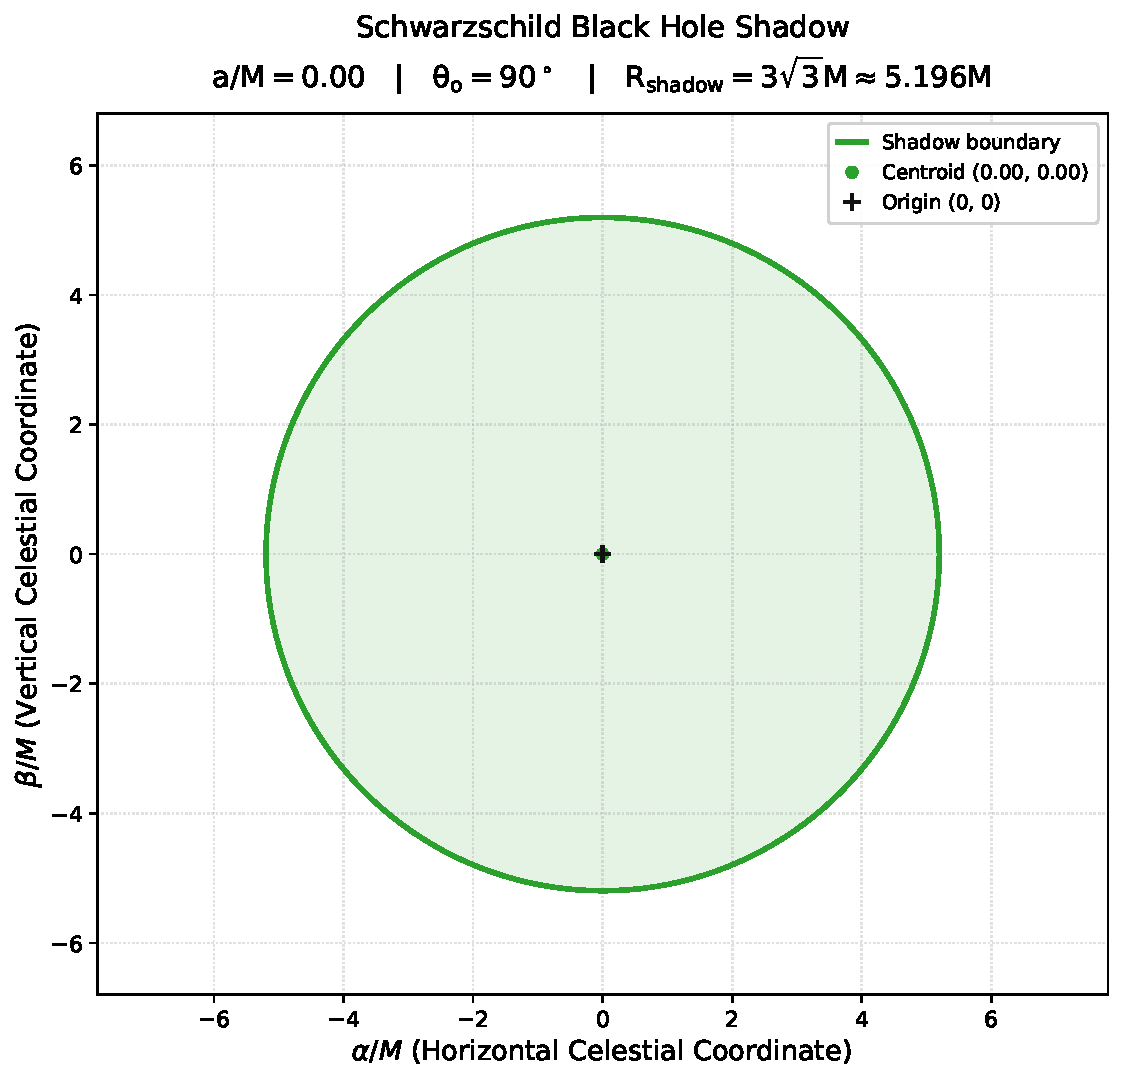
\includegraphics[width=\textwidth]{schwarzschild_shadow.pdf}
        \caption{The spherically symmetric Schwarzschild black hole shadow ($M = 1.0, a = 0$). The boundary is an exact circle centered at the origin with critical impact radius $R_{\rm circle} = 3\sqrt{3}M \approx 5.196M$ and enclosed area $A = 27\pi M^2 \approx 84.823M^2$.}
        \label{fig:schwarzschild_shadow}
    \end{minipage}
    \hfill
    \begin{minipage}[t]{0.48\textwidth}
        \centering
        \captionsetup{width=\linewidth}
        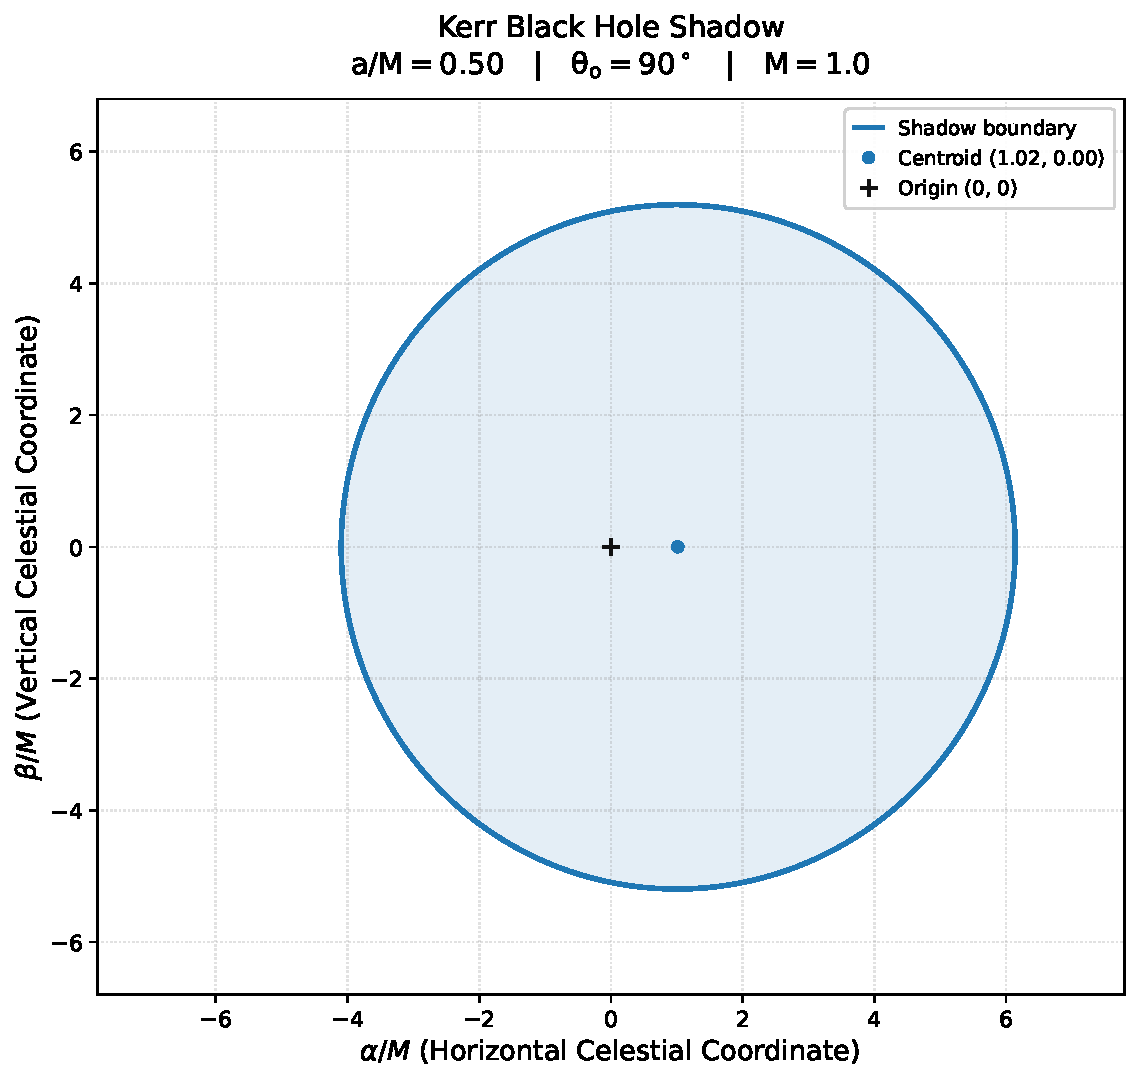
\includegraphics[width=\textwidth]{kerr_shadow_a05.pdf}
        \caption{Moderately rotating Kerr black hole shadow ($M = 1.0, a = 0.5M, \theta_o = 90^\circ$). Frame dragging shifts the retrograde boundary outwards and the prograde boundary inwards, displacing the horizontal centroid to $\bar{\alpha} = +1.02M$ while the vertical dimension remains symmetric ($A \approx 83.56M^2$).}
        \label{fig:kerr_shadow_a05}
    \end{minipage}
    \par\vspace{0.35cm}
    \begin{minipage}[t]{0.52\textwidth}
        \centering
        \captionsetup{width=\linewidth}
        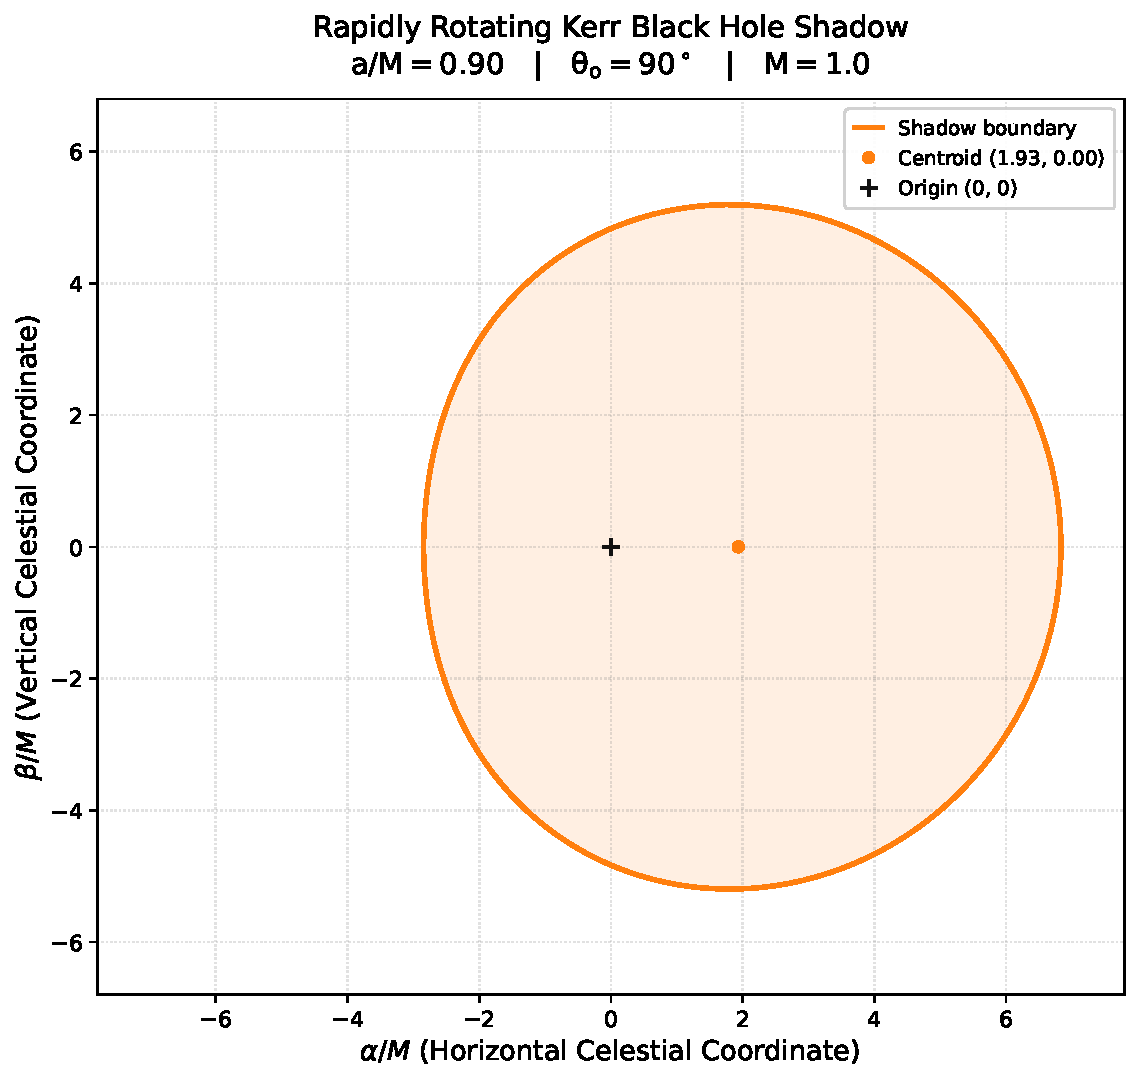
\includegraphics[width=\textwidth]{kerr_shadow_a09.pdf}
        \caption{Rapidly rotating Kerr black hole shadow ($M = 1.0, a = 0.9M, \theta_o = 90^\circ$). Strong frame-dragging shifts the prograde boundary to $\alpha_{\min} \approx -2.84M$ while the retrograde boundary extends to $\alpha_{\max} \approx +6.83M$, producing pronounced asymmetry ($A \approx 79.58M^2$, centroid $\bar{\alpha} = +1.93M$).}
        \label{fig:kerr_shadow_a09}
    \end{minipage}
\end{figure}

\subsection{Quantitative Shadow Observables Across Spin and Inclination}
\label{subsec:quantitative_shadow_observables}

To characterize the geometry of black-hole shadows quantitatively, we define five primary screen-plane observables for the closed boundary contour $\partial\Omega$ enclosing celestial region $\Omega$:
\begin{enumerate}[label=(\roman*)]
    \item \textbf{Celestial Shadow Area ($A/M^2$):}  
    The 2D planar Lebesgue measure of the shadow silhouette on the observer's screen:
    \begin{equation}
        A \equiv \iint_\Omega d\alpha\,d\beta = \frac{1}{2} \oint_{\partial\Omega} \left( \alpha\,d\beta - \beta\,d\alpha \right).
        \label{eq:area_def}
    \end{equation}
    For an open-array $N$-vertex polygon $(\alpha_i, \beta_i)_{i=0}^{N-1}$ with implicit cyclic closure $(\alpha_N, \beta_N) \equiv (\alpha_0, \beta_0)$, $A$ is evaluated via the discrete Shoelace formula:
    \begin{equation}
        A_N = \frac{1}{2} \left| \sum_{i=0}^{N-1} \left( \alpha_i \beta_{i+1} - \alpha_{i+1} \beta_i \right) \right|.
        \label{eq:shoelace_area}
    \end{equation}
    
    \item \textbf{Shadow Contour Perimeter ($P/M$):}  
    The total arc length of the closed boundary curve:
    \begin{equation}
        P \equiv \oint_{\partial\Omega} d\ell = \oint_{\partial\Omega} \sqrt{d\alpha^2 + d\beta^2}.
        \label{eq:perimeter_def}
    \end{equation}
    On the polygonal approximation, $P$ is computed by summing Euclidean chord lengths:
    \begin{equation}
        P_N = \sum_{i=0}^{N-1} \sqrt{ (\alpha_{i+1} - \alpha_i)^2 + (\beta_{i+1} - \beta_i)^2 }.
        \label{eq:polygonal_perimeter}
    \end{equation}

    \item \textbf{Horizontal Diameter ($D_{\mathrm{H}}/M$):}  
    The maximum projected extent of the shadow boundary curve parallel to the projected equatorial plane:
    \begin{equation}
        D_{\mathrm{H}} \equiv \alpha_{\max} - \alpha_{\min}.
        \label{eq:dh_def}
    \end{equation}

    \item \textbf{Vertical Diameter ($D_{\mathrm{V}}/M$):}  
    The maximum projected extent of the shadow boundary curve parallel to the projected spin axis:
    \begin{equation}
        D_{\mathrm{V}} \equiv \beta_{\max} - \beta_{\min}.
        \label{eq:dv_def}
    \end{equation}

    \item \textbf{Screen-Plane Area Centroid ($(\bar{\alpha}/M, \bar{\beta}/M)$):}  
    The center of mass of the enclosed planar domain $\Omega$:
    \begin{equation}
        \bar{\alpha} \equiv \frac{1}{A} \iint_\Omega \alpha\,d\alpha\,d\beta, \qquad
        \bar{\beta} \equiv \frac{1}{A} \iint_\Omega \beta\,d\alpha\,d\beta.
        \label{eq:centroid_def}
    \end{equation}
    Applying Green's theorem to the polygonal approximation yields the discrete moment formulas:
    \begin{align}
        \bar{\alpha}_N &= \frac{1}{6A_N} \sum_{i=0}^{N-1} (\alpha_i + \alpha_{i+1}) \left( \alpha_i \beta_{i+1} - \alpha_{i+1} \beta_i \right), \label{eq:centroid_alpha_poly} \\
        \bar{\beta}_N  &= \frac{1}{6A_N} \sum_{i=0}^{N-1} (\beta_i + \beta_{i+1}) \left( \alpha_i \beta_{i+1} - \alpha_{i+1} \beta_i \right). \label{eq:centroid_beta_poly}
    \end{align}
\end{enumerate}

\begin{table*}[t]
\centering
\small
\caption{Quantitative black hole shadow geometric observables across dimensionless spin $a/M$ and observer inclination $\theta_o$. All quantities are normalized by the black-hole mass: celestial area $A/M^2$, perimeter $P/M$, horizontal diameter $D_{\mathrm{H}}/M = \alpha_{\max} - \alpha_{\min}$, vertical diameter $D_{\mathrm{V}}/M = \beta_{\max} - \beta_{\min}$, and planar area centroid $(\bar{\alpha}/M, \bar{\beta}/M)$ computed via Green's theorem. Discrete polygonal values are evaluated at deliverable resolution $N=500$ (with $N=498$ for the piecewise-composite extremal contour). Reference values represent exact analytical limits where available (denoted with an asterisk $^*$), or independently computed high-resolution Richardson/quadrature benchmarks at $N=16\,384$. Equatorial reflection symmetry $\beta \leftrightarrow -\beta$ forces $\bar{\beta} = 0$ identically in the continuum; numerical values confirm $|\bar{\beta}_N| < 10^{-15}M$.}
\label{tab:shadow_observables}
\vspace{2mm}
\setlength{\tabcolsep}{4.5pt}
\begin{tabular}{lccccccccc}
\toprule
& & & \multicolumn{2}{c}{Area $A/M^2$} & \multicolumn{2}{c}{Perimeter $P/M$} & \multicolumn{2}{c}{Diameter $/M$} & Centroid \\
\cmidrule(lr){4-5} \cmidrule(lr){6-7} \cmidrule(lr){8-9}
Configuration & $a/M$ & $\theta_o$ & $N=500$ & Reference & $N=500$ & Reference & $D_{\mathrm{H}}$ & $D_{\mathrm{V}}$ & $\bar{\alpha}/M$ \\
\midrule
Schwarzschild & 0.00 & $90^\circ$ & 84.821 & 84.823$^*$ & 32.648 & 32.648$^*$ & 10.392 & 10.392 & 0.000 \\
Kerr & 0.50 & $90^\circ$ & 83.559 & 83.561 & 32.406 & 32.406 & 10.234 & 10.392 & 1.015 \\
Kerr & 0.90 & $90^\circ$ & 79.585 & 79.587 & 31.663 & 31.663 & 9.677 & 10.392 & 1.933 \\
Kerr & 0.90 & $45^\circ$ & 77.594 & 77.596 & 31.239 & 31.239 & 9.714 & 10.139 & 1.411 \\
Kerr & 0.90 & $15^\circ$ & 76.126 & 76.129 & 30.930 & 30.930 & 9.812 & 9.878 & 0.530 \\
Kerr (Polar) & 0.90 & $0^\circ$ & 75.923 & 75.925$^*$ & 30.888 & 30.889$^*$ & 9.832 & 9.832 & 0.000 \\
Extremal Kerr & 1.00 & $90^\circ$ & 76.243 & 76.246 & 31.177 & 31.177 & 9.000 & 10.392 & 2.288 \\
Extremal (Polar) & 1.00 & $0^\circ$ & 73.240 & 73.242$^*$ & 30.338 & 30.338$^*$ & 9.657 & 9.657 & 0.000 \\
\bottomrule
\end{tabular}
\end{table*}

\noindent \textbf{Important Methodological Distinction:} The area centroid $(\bar{\alpha}, \bar{\beta})$ must not be confused with the midpoint of the bounding box, $\left(\frac{\alpha_{\max} + \alpha_{\min}}{2}, \frac{\beta_{\max} + \beta_{\min}}{2}\right)$. Because black-hole frame dragging introduces severe left-right asymmetry, the bulk of the enclosed celestial area is weighted differently than the extremal points. For example, in rapidly rotating Kerr ($a = 0.9M, \theta_o = 90^\circ$), the bounding box midpoint lies at $\frac{6.832 - 2.844}{2} = 1.994M$, whereas the true area centroid is $\bar{\alpha} = 1.933M$, a significant physical discrepancy of $\Delta\alpha = 0.061M$.

\Cref{tab:shadow_observables} compiles the verified geometric observables across all eight standard configurations. Examination of these numerical results establishes four major relativistic trends:
\begin{enumerate}
    \item \textbf{Monotonic Area and Perimeter Contraction with Spin:}  
    At equatorial inclination ($\theta_o = 90^\circ$), increasing dimensionless spin $a/M$ from $0.00$ to $1.00$ monotonically reduces the enclosed celestial shadow area from $A = 84.823M^2$ to $76.246M^2$ (a net decrease of $10.1\%$). Similarly, the perimeter contracts monotonically from $P = 32.648M$ down to $31.177M$ (a $4.5\%$ decrease). This contraction reflects the increased binding energy and closer horizon approach permitted for prograde photon orbits.
    
    \item \textbf{Horizontal Compression and Invariance of Equatorial Vertical Diameter:}  
    As spin increases at $\theta_o = 90^\circ$, frame dragging selectively flattens the prograde boundary ($\alpha < 0$), compressing the horizontal diameter from $D_{\mathrm{H}} = 10.392M$ ($a=0$) to $D_{\mathrm{H}} = 9.677M$ ($a=0.9M$), reaching an exact integer value $D_{\mathrm{H}} = 9.000M$ in extremal Kerr ($a=1.0M$).  
    In stark contrast, the vertical diameter $D_{\mathrm{V}}$ remains rigorously invariant at:
    \begin{equation}
        D_{\mathrm{V}} = 6\sqrt{3}M \approx 10.392305M, \qquad (\theta_o = 90^\circ, \forall a \in [0, M]).
        \label{eq:dv_invariant}
    \end{equation}
    This remarkable invariance is established by distinguishing two geometric regimes. For rotating Kerr black holes ($0 < a \le M$), $\cot\theta_o = 0$ at equatorial inclination ($\theta_o = 90^\circ$), reducing \eqref{eq:bardeen_beta} to $\beta(r) = \pm\sqrt{\eta(r)}$ completely independent of $\xi(r)$. Vertical boundary extrema thus occur where $d\eta/dr = 0$. Decomposing \eqref{eq:spherical_eta} as:
    \begin{equation}
        \eta(r) = \frac{4Mr^3}{(r-M)^2} - \frac{r^4(r-3M)^2}{a^2(r-M)^2}, \qquad (0 < a \le M),
        \label{eq:eta_decomposition_kerr}
    \end{equation}
    demonstrates that both rational terms have identically vanishing radial derivatives at $r = 3M$, yielding $\eta(3M) = 27M^2$, $\eta'(3M) = 0$, and $\eta''(3M) < 0$. This establishes $\beta_{\max} = \sqrt{27}M = 3\sqrt{3}M$ and $D_{\mathrm{V}} = 2\beta_{\max} = 6\sqrt{3}M$, with horizontal coordinate $\alpha = -\xi(3M) = +2a$ displaced toward the retrograde screen hemisphere. In the non-rotating Schwarzschild limit ($a = 0$), where the $1/a^2$ factor is formally singular, spherical symmetry independently dictates that the shadow is an exact circle of radius $R_{\rm circle} = 3\sqrt{3}M \approx 5.196M$ (cf.~Section~\ref{subsec:schwarzschild_photon_sphere}), establishing identically $D_{\mathrm{V}} = 2 R_{\rm circle} = 6\sqrt{3}M$. As $a \to 0$, the horizontal displacement $\alpha = +2a$ continuously tends to zero, smoothly recovering the unshifted, symmetric Schwarzschild boundary vertices at $(\alpha, \beta) = (0, \pm 3\sqrt{3}M)$.

    \item \textbf{Retrograde Centroid Displacement:}  
    Because $\alpha = -\xi/\sin\theta_o$, prograde photon orbits ($\xi > 0$) map to the negative $\alpha$ hemisphere, whereas retrograde orbits ($\xi < 0$) map to the positive $\alpha$ hemisphere. Prograde orbits can orbit much closer to the horizon ($r_{\rm ph}^+ \to M$), requiring smaller impact parameters and compressing the prograde boundary to $\alpha_{\min} \ge -2M$. Retrograde orbits remain distant ($r_{\rm ph}^- \to 4M$), extending the retrograde boundary to $\alpha_{\max} = +7M$ in extremal Kerr. Consequently, frame dragging shifts the centroid systematically toward the positive (retrograde) screen coordinate, increasing from $\bar{\alpha} = 0.000M$ to $+1.015M$ ($a=0.5M$), $+1.933M$ ($a=0.9M$), and $+2.288M$ ($a=1.0M$).

    \item \textbf{Smooth Circular Restoration Across Observer Inclinations:}  
    For a rapidly rotating black hole ($a=0.9M$), decreasing observer inclination from edge-on ($\theta_o = 90^\circ$) to face-on ($\theta_o = 0^\circ$) systematically eliminates the projected frame-dragging distortion. The centroid displacement $\bar{\alpha}$ smoothly subsides from $+1.933M$ ($\theta_o=90^\circ$) to $+1.411M$ ($45^\circ$), $+0.530M$ ($15^\circ$), and vanishes identically at $\theta_o = 0^\circ$. Simultaneously, $D_{\mathrm{H}}$ and $D_{\mathrm{V}}$ converge from an aspect ratio of $D_{\mathrm{H}}/D_{\mathrm{V}} \approx 0.931$ to an exact circle with $D_{\mathrm{H}} = D_{\mathrm{V}} = 9.832M$.
\end{enumerate}

\section{Polar Observers, Extremal Kerr and NHEK Structure}
\label{sec:extremal_nhek_and_polar}

\subsection{Extremal Kerr Black Holes and the Critical Inclination}
\label{subsec:extremal_kerr_critical}
In the extreme Kerr limit ($|a| = M$), the outer event horizon and inner Cauchy horizon coalesce at coordinate radius $r_+ = r_- = M$. The metric horizon function $\Delta(r) = (r - M)^2$ develops a double root, and the exterior spherical photon orbit parameters \eqref{eq:spherical_xi}--\eqref{eq:spherical_eta} simplify to:
\begin{align}
    \xi_{\rm ext}(r) &= M + 2r - \frac{r^2}{M}, \label{eq:extremal_xi} \\
    \eta_{\rm ext}(r) &= \frac{r^3\left[4M^3 - r(r - 3M)^2\right]}{M^2(r - M)^2}. \label{eq:extremal_eta}
\end{align}
As the generating spherical orbit approaches the horizon from the exterior ($r \to M^+$), these parameters approach finite, non-zero limiting values:
\begin{equation}
    \lim_{r \to M^+} \xi_{\rm ext}(r) = 2M, \qquad \lim_{r \to M^+} \eta_{\rm ext}(r) = 3M^2.
    \label{eq:extremal_horizon_limits}
\end{equation}

Evaluating the Carter vertical radicand function $B(r; \theta_o)$ defined in \eqref{eq:carter_B_u} directly at the horizon $r = M$ yields:
\begin{equation}
    B(M; \theta_o) = 3M^2 + M^2\cos^2\theta_o - 4M^2\cot^2\theta_o = M^2 \left( 3 - C(\theta_o) \right),
    \label{eq:B_horizon_extremal}
\end{equation}
where the inclination function $C(\theta_o)$ is:
\begin{equation}
    C(\theta_o) \equiv \frac{\cos^2\theta_o \left(3 + \cos^2\theta_o\right)}{\sin^2\theta_o} \ge 0.
    \label{eq:def_C_theta}
\end{equation}
The physical existence of real shadow boundary points requires $B(M; \theta_o) \ge 0$, which is satisfied if and only if $C(\theta_o) \le 3$. Setting $C(\theta_{\rm crit}) = 3$ yields a quadratic equation in $\cos^2\theta_{\rm crit}$:
\begin{equation}
    \cos^4\theta_{\rm crit} + 6\cos^2\theta_{\rm crit} - 3 = 0 \implies \cos^2\theta_{\rm crit} = 2\sqrt{3} - 3 \approx 0.4641016,
    \label{eq:theta_crit_derivation}
\end{equation}
defining the critical observer inclination $\theta_{\rm crit}$ \cite{Bardeen1973,Gralla2020}:
\begin{equation}
    \theta_{\rm crit} = \arccos\left(\sqrt{2\sqrt{3} - 3}\right) \approx 47.058597^\circ \approx 0.821323 \text{ rad}.
    \label{eq:theta_crit_val}
\end{equation}

\subsection{Near-Horizon Extreme Kerr (NHEK) Vertical Segment}
\label{subsec:nhek_vertical_segment}
The critical angle $\theta_{\rm crit}$ partitions the observational phenomenology of extremal Kerr black holes into two distinct geometric regimes:
\begin{enumerate}
    \item \textbf{Subcritical Observers ($\theta_o < \theta_{\rm crit}$):}  
    For inclinations closer to the pole than $\theta_{\rm crit}$, $C(\theta_o) > 3$, implying $B(M; \theta_o) < 0$. The turning points $B(r; \theta_o) = 0$ occur strictly exterior to the horizon ($r_{\min} > M$). The shadow boundary is closed, strictly convex, and smooth, with the event horizon completely shielded from direct celestial view by the photon capture barrier.
    
    \item \textbf{Supercritical Observers ($\theta_o > \theta_{\rm crit}$, e.g., Equatorial $\theta_o = 90^\circ$):}  
    For inclinations closer to the equator than $\theta_{\rm crit}$, $C(\theta_o) < 3$, so $B(M; \theta_o) > 0$. The exterior curved boundary reaches the horizon at $r = M$, terminating at horizontal impact coordinate:
    \begin{equation}
        \alpha_{\rm pro} = -\frac{\xi_{\rm ext}(M)}{\sin\theta_o} = -\frac{2M}{\sin\theta_o},
    \end{equation}
    with non-zero vertical coordinate $\pm \beta_{\max}$, where:
    \begin{equation}
        \beta_{\max} \equiv M \sqrt{3 - C(\theta_o)}.
        \label{eq:beta_max_nhek}
    \end{equation}
\end{enumerate}

To complete the closed boundary of the shadow, the termination points $(\alpha_{\rm pro}, \pm\beta_{\max})$ are joined by an exact vertical line segment:
\begin{equation}
    \alpha_{\rm NHEK} = -\frac{2M}{\sin\theta_o}, \qquad \beta \in [-\beta_{\max}, +\beta_{\max}].
    \label{eq:nhek_line_segment}
\end{equation}
Physically, this straight segment represents the projection of an infinite family of bound spherical photon orbits that reside on the infinitely extended throat of the Near-Horizon Extreme Kerr (NHEK) geometry \cite{BardeenPressTeukolsky1972,Gralla2020}. In the extremal limit, the coordinate distance to the horizon collapses, but the physical proper distance blows up, opening an infinite throat endowed with an enhanced $SL(2, \mathbb{R}) \times U(1)$ conformal isometry group. Photons with $\xi = 2M$ and Carter constants $\eta \in [4M^2\cot^2\theta_o - M^2\cos^2\theta_o, 3M^2]$ reside on radially unstable spherical photon orbits (separatrices) within this throat (with $\eta = 3M^2$ forming the marginally degenerate endpoint where $R''(M) = 0$), casting an exact vertical line on the observer's screen.

For an equatorial observer ($\theta_o = 90^\circ$), $C(\pi/2) = 0$, giving:
\begin{equation}
    \alpha_{\rm NHEK} = -2M, \qquad \beta \in [-\sqrt{3}M, +\sqrt{3}M],
    \label{eq:nhek_equatorial}
\end{equation}
forming the characteristic flat D-shaped vertical edge shown in \Cref{fig:kerr_shadow_extremal}.

\begin{figure}[!htbp]
    \centering
    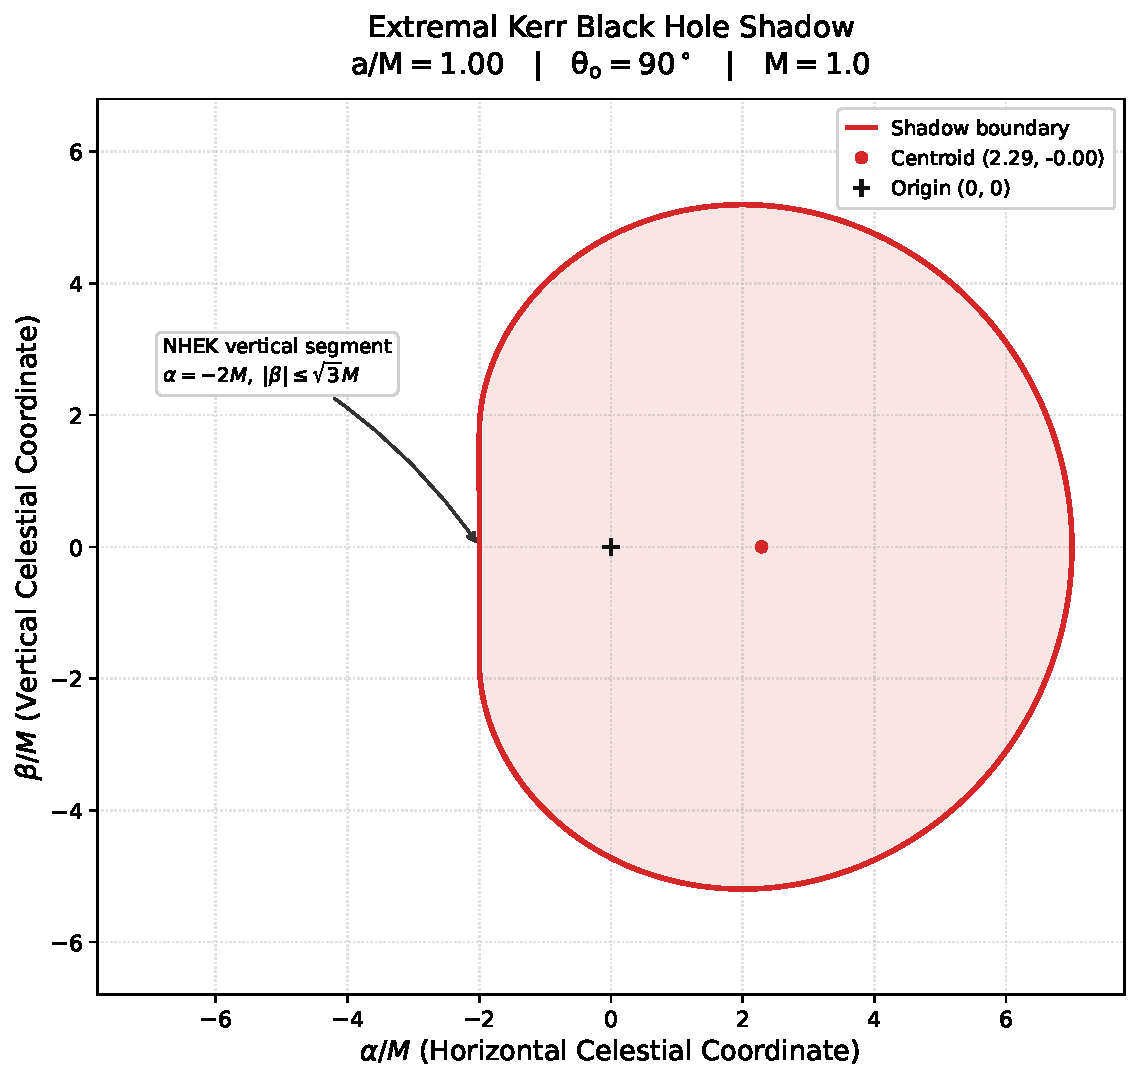
\includegraphics[width=0.58\textwidth]{kerr_shadow_extremal.pdf}
    \caption{Extremal Kerr black hole shadow ($M = 1.0, a = 1.0M, \theta_o = 90^\circ$). The prograde boundary is terminated by the vertical Near-Horizon Extreme Kerr (NHEK) line segment at $\alpha = -2M$, spanning $\beta \in [-\sqrt{3}M, +\sqrt{3}M]$ ($\beta_{\max} \approx 1.732M$), joining the smooth exterior curved branch at sharp $C^0$ corners.}
    \label{fig:kerr_shadow_extremal}
\end{figure}

\subsection{Multi-Inclination Comparison for Rapidly Rotating Black Holes}
\label{subsec:inclination_comparison}
The appearance of a black-hole shadow depends sensitively on the observer's line-of-sight inclination $\theta_o$. \Cref{fig:kerr_shadow_inclination_comparison} presents the verified shadow profiles for a rapidly rotating Kerr black hole ($a = 0.90M, M = 1.0$) across three representative observer inclinations:
\begin{equation}
    \theta_o \in \{15^\circ, 45^\circ, 90^\circ\}.
\end{equation}

\begin{figure}[!htbp]
    \centering
    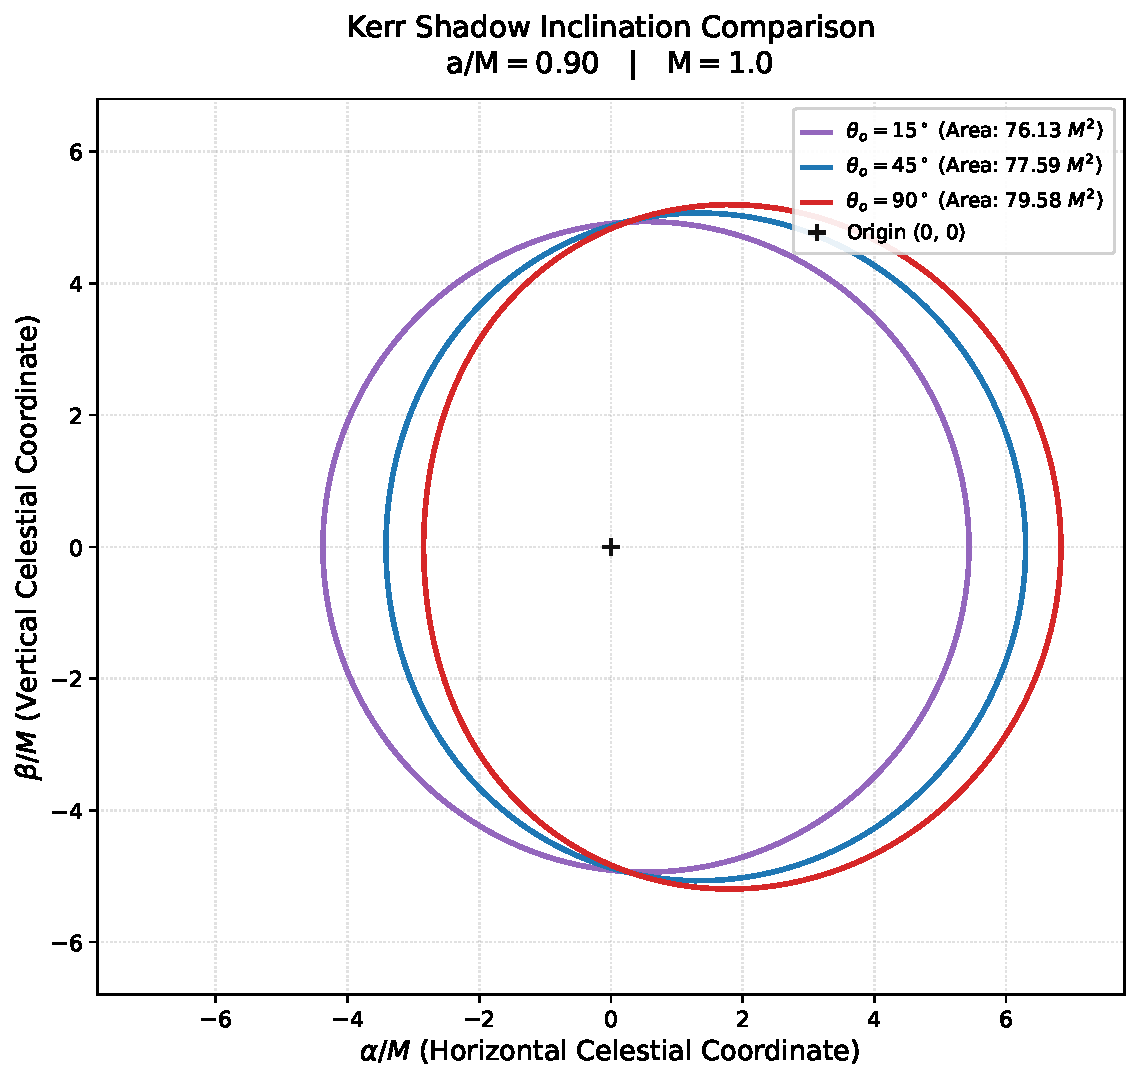
\includegraphics[width=0.58\textwidth]{kerr_shadow_inclination_comparison.pdf}
    \caption{Comparison of Kerr black hole shadow boundaries at $a/M = 0.90$ across observer inclinations $\theta_o = 15^\circ$ ($A = 76.13M^2$), $\theta_o = 45^\circ$ ($A = 77.59M^2$), and $\theta_o = 90^\circ$ ($A = 79.58M^2$). The profile transitions smoothly from an asymmetric, flattened D-shape at high inclination to a nearly circular silhouette near the pole.}
    \label{fig:kerr_shadow_inclination_comparison}
\end{figure}

The physical progression across inclinations exhibits clear geometric systematics:
\begin{itemize}
    \item \textbf{Equatorial Observer ($\theta_o = 90^\circ$):} The line of sight lies directly in the black hole's equatorial plane. Frame-dragging is maximally projected onto the celestial screen ($\sin\theta_o = 1$). Prograde photons can orbit as close as $r_{\rm ph}^+ \approx 1.56M$, compressing the prograde edge to $\alpha_{\min} \approx -2.84M$, whereas retrograde photons are held out at $r_{\rm ph}^- \approx 3.91M$, extending the retrograde edge to $\alpha_{\max} \approx +6.83M$. This creates maximal horizontal asymmetry ($D_{\mathrm{H}} = 9.68M, D_{\mathrm{V}} = 10.39M$), with the area centroid displaced to $\bar{\alpha} = +1.93M$.
    \item \textbf{Intermediate Observer ($\theta_o = 45^\circ$):} Because the projected spin vector is inclined by $45^\circ$, the asymmetric displacement of the centroid decreases to $\bar{\alpha} = +1.41M$, and the enclosed area contracts to $A = 77.59M^2$.
    \item \textbf{Near-Polar Observer ($\theta_o = 15^\circ$):} As the observer approaches the rotation axis, the apparent velocity of spacetime rotation projected perpendicular to the line of sight diminishes proportionally to $\sin\theta_o$. The centroid shift drops to $\bar{\alpha} = +0.53M$, and the horizontal and vertical diameters become nearly equal ($D_{\mathrm{H}} = 9.81M, D_{\mathrm{V}} = 9.88M$), yielding a nearly circular silhouette ($A = 76.13M^2$).
\end{itemize}

\subsection{Exact-Polar Observer Shadows ($\theta_o = 0^\circ$)}
\label{subsec:exact_polar_shadows}
For an observer situated precisely on the polar rotation axis ($\theta_o = 0^\circ$), axial symmetry requires that the black-hole shadow must be an exact circle centered at the origin of the celestial screen ($\alpha^2 + \beta^2 = R_{\rm pole}^2$).

In the polar limit $\theta_o \to 0$, $\cot^2\theta_o \to \infty$. To prevent the vertical radicand $\beta^2 = \eta + a^2\cos^2\theta_o - \xi^2\cot^2\theta_o$ from diverging to $-\infty$, the axial angular momentum of the generating spherical photon orbit must vanish identically:
\begin{equation}
    \xi(r_p) = 0 \iff M(r_p^2 - a^2) - r_p\Delta(r_p) = 0 \iff r_p^2(3M - r_p) - a^2(r_p + M) = 0.
    \label{eq:polar_orbit_equation}
\end{equation}
For any spin $a \in [0, M]$, \eqref{eq:polar_orbit_equation} has a unique physical root $r_p$ in the exterior interval $(M, 3M]$:
\begin{equation}
    r_p \in [1 + \sqrt{2}, 3]M.
    \label{eq:rp_range}
\end{equation}
At this polar radius, the Carter constant $\eta_p \equiv \eta(r_p)$ is strictly positive. Evaluating the screen radius in the limit $\theta_o \to 0$ gives:
\begin{equation}
    R_{\rm pole}(a) \equiv \sqrt{\eta(r_p) + a^2}.
    \label{eq:polar_circle_radius}
\end{equation}

\subsubsection{Derivation of the Polar Extremal Shadow Radius}
For an extremal black hole ($a = M$), \eqref{eq:polar_orbit_equation} becomes:
\begin{equation}
    r_p^2(3M - r_p) - M^2(r_p + M) = 0 \iff r_p^3 - 3M r_p^2 + M^2 r_p + M^3 = 0.
    \label{eq:extremal_polar_poly}
\end{equation}
Factoring out the root at $r = M$ gives:
\begin{equation}
    (r_p - M)\left( r_p^2 - 2M r_p - M^2 \right) = 0 \iff (r_p - M)\left[ (r_p - M)^2 - 2M^2 \right] = 0.
\end{equation}
The unique root exterior to the horizon ($r_p > M$) is:
\begin{equation}
    r_p = (1 + \sqrt{2})M \approx 2.41421356M.
    \label{eq:rp_extremal_val}
\end{equation}

To evaluate the Carter constant $\eta(r_p)$ at this radius, we introduce the dimensionless radial coordinate $x \equiv r/M$, so that the extremal Carter constant \eqref{eq:extremal_eta} takes the form:
\begin{equation}
    \frac{\eta_{\rm ext}(r)}{M^2} = \frac{x^3\left[ 4 - x(x - 3)^2 \right]}{(x - 1)^2}.
    \label{eq:extremal_eta_dimensionless}
\end{equation}
At the polar photon orbit, $x_p \equiv r_p/M = 1 + \sqrt{2}$. We evaluate each component systematically:
\begin{align}
    (x_p - 1)^2 &= \left(\sqrt{2}\right)^2 = 2, \label{eq:eval_denom} \\
    x_p^3 &= (1 + \sqrt{2})^3 = 1 + 3\sqrt{2} + 6 + 2\sqrt{2} = 7 + 5\sqrt{2}, \label{eq:eval_cube} \\
    x_p - 3 &= \sqrt{2} - 2 \implies (x_p - 3)^2 = 2 - 4\sqrt{2} + 4 = 6 - 4\sqrt{2}, \label{eq:eval_sq} \\
    x_p(x_p - 3)^2 &= (1 + \sqrt{2})(6 - 4\sqrt{2}) = 6 - 4\sqrt{2} + 6\sqrt{2} - 8 = -2 + 2\sqrt{2}, \label{eq:eval_prod} \\
    4 - x_p(x_p - 3)^2 &= 4 - (-2 + 2\sqrt{2}) = 6 - 2\sqrt{2}. \label{eq:eval_bracket}
\end{align}
Multiplying the cubic prefactor \eqref{eq:eval_cube} by the bracket \eqref{eq:eval_bracket} gives the numerator:
\begin{equation}
    x_p^3\left[ 4 - x_p(x_p - 3)^2 \right] = (7 + 5\sqrt{2})(6 - 2\sqrt{2}) = 42 - 14\sqrt{2} + 30\sqrt{2} - 20 = 22 + 16\sqrt{2}.
\end{equation}
Dividing by the denominator $(x_p - 1)^2 = 2$ from \eqref{eq:eval_denom} yields the exact Carter constant:
\begin{equation}
    \eta_{\rm ext}(r_p) = \frac{22 + 16\sqrt{2}}{2} M^2 = (11 + 8\sqrt{2}) M^2.
    \label{eq:eta_extremal_polar}
\end{equation}

The polar shadow screen radius is therefore:
\begin{align}
    R_{\rm pole}^2 &= \eta_{\rm ext}(r_p) + a^2 = (11 + 8\sqrt{2})M^2 + M^2 = (12 + 8\sqrt{2})M^2 \nonumber \\
    &= 4\left(3 + 2\sqrt{2}\right)M^2 = 4\left(1 + \sqrt{2}\right)^2 M^2.
    \label{eq:R_pole_squared_derivation}
\end{align}
Taking the positive square root yields the exact analytical result:
\begin{equation}
    R_{\rm pole}(M) = 2\left(1 + \sqrt{2}\right)M = \sqrt{12 + 8\sqrt{2}}M \approx 4.82842712M.
    \label{eq:R_pole_extremal_exact}
\end{equation}
Notice that $R_{\rm pole}(M) = 2 r_p$. The corresponding diameters and celestial area are:
\begin{align}
    D_{\mathrm{H}} &= D_{\mathrm{V}} = 2 R_{\rm pole} = 4\left(1 + \sqrt{2}\right)M \approx 9.656854M, \label{eq:extremal_polar_diameters} \\
    A &= \pi R_{\rm pole}^2 = 4\left(3 + 2\sqrt{2}\right)\pi M^2 \approx 73.2415M^2, \label{eq:extremal_polar_area}
\end{align}
matching the underlying high-resolution numerical observables to eight significant digits, consistent with the displayed values in \Cref{tab:shadow_observables}.

In the Schwarzschild limit ($a = 0$), $r_p = 3M$ and $\eta(3M) = 27M^2$, giving $R_{\rm pole}(0) = 3\sqrt{3}M \approx 5.196152M$. \Cref{fig:exact_polar_shadow} presents the verified polar shadow circles across spins $a/M \in \{0.0, 0.5, 0.9, 1.0\}$, demonstrating the monotonic contraction of the circular shadow radius from $3\sqrt{3}M \approx 5.196M$ down to $2(1+\sqrt{2})M \approx 4.828M$ as spin approaches extremality.

\begin{figure}[!htbp]
    \centering
    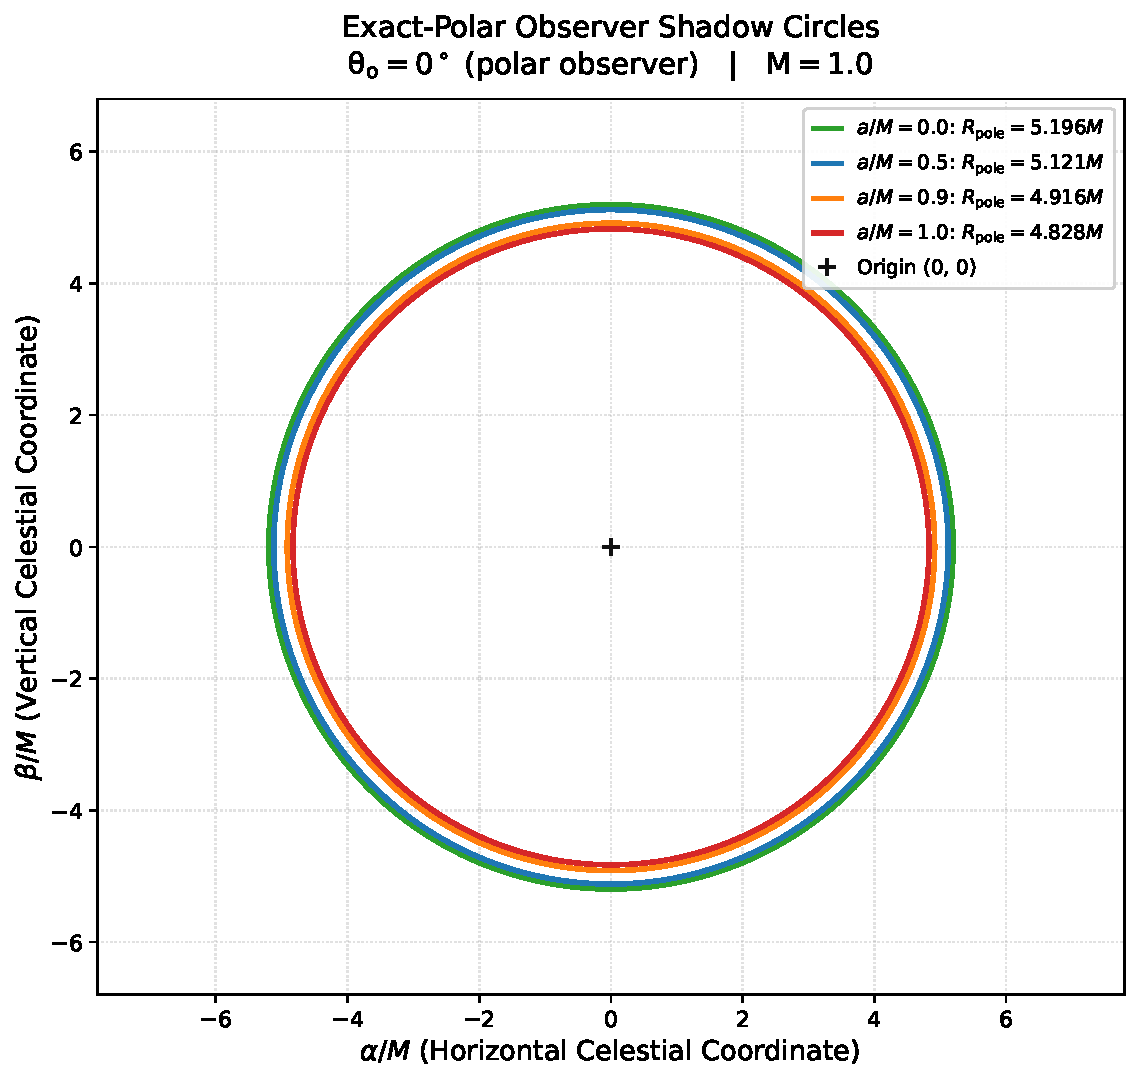
\includegraphics[width=0.58\textwidth]{exact_polar_shadow.pdf}
    \caption{Exact-polar observer shadow boundaries ($\theta_o = 0^\circ$) across black hole spins $a/M \in \{0.0, 0.5, 0.9, 1.0\}$. All boundaries are concentric circles centered at the origin, with radii contracting monotonically from $R_{\rm pole} = 3\sqrt{3}M \approx 5.196M$ ($a=0$) down to $R_{\rm pole} = 2(1+\sqrt{2})M \approx 4.828M$ ($a=M$).}
    \label{fig:exact_polar_shadow}
\end{figure}

\section{Near-Polar Asymptotic Analysis}
\label{sec:near_polar_asymptotics}

\subsection{Endpoint Perturbation Expansions}
When the observer polar inclination is near the rotation axis ($\theta_o \ll 1$), the celestial screen coordinates undergo small geometric perturbations away from the exact polar circle. Let:
\begin{equation}
    s \equiv \sin\theta_o \ll 1, \qquad c \equiv \cos\theta_o = \sqrt{1 - s^2}.
\end{equation}
The boundary turning points correspond to roots of the Carter vertical function $B(r; \theta_o) = 0$:
\begin{equation}
    (1 - s^2) \xi(r)^2 = s^2 \left[ \eta(r) + a^2(1 - s^2) \right].
    \label{eq:turning_point_governing_eq}
\end{equation}

Let $r_p$ be the polar radius defined by $\xi(r_p) = 0$, and define the expansion derivatives:
\begin{equation}
    k \equiv \xi'(r_p), \quad l \equiv \xi''(r_p), \quad e \equiv \eta'(r_p), \quad R_p \equiv \sqrt{\eta(r_p) + a^2}.
    \label{eq:asymptotic_derivative_defs}
\end{equation}
For all $a > 0$, since $r_p \in [1+\sqrt{2}, 3]M > 2M$, the numerator satisfies $6Mr_p - 3r_p^2 - a^2 = -3r_p(r_p - 2M) - a^2 < 0$, ensuring $k = \frac{6Mr_p - 3r_p^2 - a^2}{a(r_p - M)} < 0$ (so $|k| = -k \neq 0$).

Expanding $\Delta r \equiv r - r_p = s\,z_1 + s^2 z_2 + \mathcal{O}(s^3)$ in \eqref{eq:turning_point_governing_eq} yields at order $s^2$:
\begin{equation}
    k^2 z_1^2 = R_p^2 \implies z_1 = \pm \frac{R_p}{|k|}.
\end{equation}
Defining the scale amplitude:
\begin{equation}
    A \equiv \frac{R_p}{|k|} = -\frac{R_p}{k} > 0,
    \label{eq:def_scale_amplitude_A}
\end{equation}
the outer and inner radial turning points are $r_{\max} = r_p + s A + \mathcal{O}(s^2)$ and $r_{\min} = r_p - s A + \mathcal{O}(s^2)$.

At order $s^3$, matching terms yields $2k^2 z_1 z_2 + k l z_1^3 = e z_1$. Dividing by $z_1 = \pm A \neq 0$:
\begin{equation}
    2k^2 z_2 + k l A^2 = e \implies \boxed{z_2 = \frac{k e - l R_p^2}{2k^3}}.
    \label{eq:z2_exact_formula}
\end{equation}
Because $z_1^2 = A^2$ is independent of the sign of $z_1$, the second-order displacement $z_2$ is identical for both turning points:
\begin{align}
    r_{\max} &= r_p + s A + s^2 z_2 + \mathcal{O}(s^3), \label{eq:r_max_expansion} \\
    r_{\min} &= r_p - s A + s^2 z_2 + \mathcal{O}(s^3). \label{eq:r_min_expansion}
\end{align}
The midpoint displacement satisfies $r_{\rm mid} - r_p = \frac{1}{2}(r_{\max} + r_{\min}) - r_p = s^2 z_2 + \mathcal{O}(s^4)$ (strictly $\mathcal{O}(s^2)$).

\subsection{Full Screen-Coordinate Perturbation Expansions}
Parameterizing the radial coordinate smoothly as $r(\phi) = r_{\rm mid} - r_{\rm amp}\cos\phi$ on $\phi \in [0, \pi]$ (where $\phi \mapsto \pi - \phi$ relative to Section~\ref{subsec:smooth_contour} so that $\phi = 0$ corresponds to $r_{\min}$ and $\phi = \pi$ to $r_{\max}$):
\begin{equation}
    r(\phi) - r_p = -s A \cos\phi + s^2 z_2 + \mathcal{O}(s^3).
\end{equation}

\subsubsection{Horizontal Coordinate $\alpha(\phi)$}
Taylor expanding $\xi(r(\phi))$ about $r_p$:
\begin{align}
    \xi(r(\phi)) &= k\left(-s A \cos\phi + s^2 z_2\right) + \frac{1}{2}l\left(-s A \cos\phi\right)^2 + \mathcal{O}(s^3) \nonumber \\
    &= -s k A \cos\phi + s^2 \left( k z_2 + \frac{1}{2} l A^2 \cos^2\phi \right) + \mathcal{O}(s^3).
\end{align}
Using $k A = -R_p$ and dividing by $-s$:
\begin{equation}
    \alpha(\phi) = -\frac{\xi(r(\phi))}{s} = -R_p\cos\phi - s\left( k z_2 + \frac{1}{2} l A^2 \cos^2\phi \right) + \mathcal{O}(s^2).
\end{equation}
Applying the double-angle identity $\cos^2\phi = \frac{1 + \cos(2\phi)}{2}$:
\begin{equation}
    \boxed{\alpha(\phi) = -R_p\cos\phi + s\,\delta_0 - s\,\lambda\cos(2\phi) + \mathcal{O}(s^2)},
    \label{eq:alpha_asymptotic_expansion}
\end{equation}
where the first-order deformation and shift coefficients are:
\begin{align}
    \lambda &\equiv \frac{1}{4} l A^2 = \frac{l R_p^2}{4k^2}, \label{eq:def_lambda} \\
    \delta_0 &\equiv -\left(k z_2 + \lambda\right) = -\frac{k e - \frac{1}{2} l R_p^2}{2k^2}. \label{eq:def_delta0}
\end{align}
Evaluating the planar area centroid via Green's theorem $\bar{\alpha} = \frac{1}{2A}\oint \alpha^2 d\beta$ confirms that the quadrupole $\lambda$ cancels identically, yielding the exact first-order horizontal centroid displacement:
\begin{equation}
    \boxed{\bar{\alpha} = s\left(\delta_0 - \lambda\right) + \mathcal{O}(s^2) = -s\frac{\eta'(r_p)}{2\xi'(r_p)} + \mathcal{O}(s^2)}.
    \label{eq:near_polar_centroid_shift}
\end{equation}

\subsubsection{Signed Vertical Coordinate $\beta(\phi)$}
The squared vertical coordinate is $\beta(\phi)^2 = \eta(r(\phi)) + a^2(1 - s^2) - \frac{1 - s^2}{s^2}\xi(r(\phi))^2$. Expanding both contributions:
\begin{align}
    \eta(r(\phi)) + a^2(1 - s^2) &= R_p^2 - s e A \cos\phi + \mathcal{O}(s^2), \\
    -\frac{1 - s^2}{s^2}\xi(r(\phi))^2 &= -R_p^2\cos^2\phi - 2s R_p\cos\phi \left( k z_2 + \frac{1}{2} l A^2 \cos^2\phi \right) + \mathcal{O}(s^2).
\end{align}
Adding yields $\beta(\phi)^2 = R_p^2(1 - \cos^2\phi) + s K_1(\phi) + \mathcal{O}(s^2) = R_p^2\sin^2\phi + s K_1(\phi) + \mathcal{O}(s^2)$, where:
\begin{equation}
    K_1(\phi) \equiv -e A \cos\phi - 2 R_p\cos\phi \left( k z_2 + \frac{1}{2} l A^2 \cos^2\phi \right).
    \label{eq:K1_def}
\end{equation}
From the order-$s^3$ endpoint condition, $2k^2 z_2 + l A^2 k = e$. Multiplying by $A = -R_p/k$:
\begin{equation}
    -e A = +2 R_p \left( k z_2 + \frac{1}{2} l A^2 \right).
\end{equation}
Substituting into $K_1(\phi)$ eliminates the uncoupled $\cos\phi$ term:
\begin{equation}
    K_1(\phi) = \cos\phi \left[ 2 R_p k z_2 + l R_p A^2 - 2 R_p k z_2 - l R_p A^2 \cos^2\phi \right] = l R_p A^2 \cos\phi \sin^2\phi.
    \label{eq:K1_simplified}
\end{equation}
Because $\sin^2\phi$ factors globally out of $\beta(\phi)^2$, the square root is extracted without division by $\sin\phi$:
\begin{equation}
    \beta_{\rm upper}(\phi) = \sin\phi \cdot R_p \sqrt{1 + s \frac{l A^2}{R_p}\cos\phi + \mathcal{O}(s^2)} = R_p\sin\phi + \frac{1}{2} s l A^2 \sin\phi\cos\phi + \mathcal{O}(s^2).
\end{equation}
Using $\sin\phi\cos\phi = \frac{1}{2}\sin(2\phi)$ and $\lambda = \frac{1}{4} l A^2$, and recognizing that the lower branch $\beta \le 0$ matches $-\sin\phi = |\sin\phi|$ on $[\pi, 2\pi]$, we obtain the \textbf{signed, uniformly valid representation over $\phi \in [0, 2\pi]$}:
\begin{equation}
    \boxed{\beta(\phi) = R_p\sin\phi + s\,\lambda\sin(2\phi) + \mathcal{O}(s^2)}.
    \label{eq:beta_asymptotic_expansion}
\end{equation}

\subsection{Speed Dipole, Curvature Invariance, and First-Order Invariance}
Differentiating \eqref{eq:alpha_asymptotic_expansion} and \eqref{eq:beta_asymptotic_expansion} with respect to $\phi$:
\begin{align}
    \alpha'(\phi) &= R_p\sin\phi + 2s\lambda\sin(2\phi) + \mathcal{O}(s^2), \label{eq:dalpha_dphi} \\
    \beta'(\phi) &= R_p\cos\phi + 2s\lambda\cos(2\phi) + \mathcal{O}(s^2). \label{eq:dbeta_dphi}
\end{align}
Evaluating the squared metric speed $\sigma(\phi)^2 = \alpha'(\phi)^2 + \beta'(\phi)^2$:
\begin{equation}
    \sigma(\phi)^2 = R_p^2 + 4s\lambda R_p \left(\sin\phi\sin(2\phi) + \cos\phi\cos(2\phi)\right) + \mathcal{O}(s^2) = R_p^2 + 4s\lambda R_p \cos\phi + \mathcal{O}(s^2).
\end{equation}
Taking the square root:
\begin{equation}
    \boxed{\sigma(\phi) = R_p + 2s\lambda\cos\phi + \mathcal{O}(s^2)}.
    \label{eq:speed_dipole}
\end{equation}
The metric speed forms a \textbf{pure $\cos\phi$ dipole} to first order in inclination.

Computing the planar curvature magnitude:
\begin{equation}
    \kappa(\phi) \equiv \frac{|\alpha'\beta'' - \beta'\alpha''|}{\sigma^3} = \frac{R_p^2 + 6s\lambda R_p\cos\phi + \mathcal{O}(s^2)}{R_p^3 + 6s\lambda R_p^2\cos\phi + \mathcal{O}(s^2)} = \boxed{R_p^{-1} + \mathcal{O}(s^2)}.
    \label{eq:curvature_invariance}
\end{equation}
The linear harmonic cancels identically between numerator and denominator, proving that \textbf{planar curvature magnitude is invariant to first order in inclination}.

Integrating over $\phi \in [0, 2\pi]$, dipole orthogonality ($\int_0^{2\pi} \cos\phi\,d\phi = 0$) ensures:
\begin{align}
    P_{\rm cont}(s) - 2\pi R_p &= \int_0^{2\pi} \left(2s\lambda\cos\phi + \mathcal{O}(s^2)\right) d\phi = \boxed{\mathcal{O}(s^2)}, \label{eq:P_cont_invariance} \\
    \mathcal{I}(s) - 2\pi R_p &= \int_0^{2\pi} \left(6s\lambda\cos\phi + \mathcal{O}(s^2)\right) d\phi = \boxed{\mathcal{O}(s^2)}, \label{eq:I_functional_invariance}
\end{align}
establishing that the continuous perimeter and the curvature functional are invariant to first order in observer inclination.

\subsection{Global Polygonal Chord Error Formulation}
For a $C^4$ closed curve with nowhere-vanishing metric speed ($\sigma > 0$), symmetric midpoint Euler--Maclaurin summation of chord lengths $\Delta\mathbf{r}_j = \mathbf{r}(\phi_j + h/2) - \mathbf{r}(\phi_j - h/2)$ with $h = 2\pi/N$ yields:
\begin{equation}
    \boxed{P_N - P_{\rm cont} = -\frac{h^2}{24}\mathcal{I} + \mathcal{O}(h^4) = -\frac{\pi^2}{6N^2}\mathcal{I} + \mathcal{O}(N^{-4})},
    \label{eq:polygonal_chord_error_formula}
\end{equation}
where $\mathcal{I} \equiv \int_0^{2\pi} \kappa^2 \sigma^3\,d\phi$, with circular limit $\mathcal{I}_{\rm circle} = 2\pi R_p$ carrying dimensions of length $[L]$.

\subsection{Scope and Regularity Assumptions}
The mathematical validity of the near-polar expansions is subject to three specific regularity qualifications:
\begin{enumerate}
    \item \textbf{Joint Smooth Extension Assumption:} Uniform bounds on derivatives ($\|R_\alpha''\|_{C^0} = \mathcal{O}(s^2), \|R_\beta''\|_{C^0} = \mathcal{O}(s^2)$) require the endpoint-remapped coordinates to admit a jointly smooth extension in $(s, \phi)$ through $s = 0$, which is formally classified as a required regularity assumption.
    \item \textbf{Fixed-Spin Validity:} Denominators remain non-zero for each fixed $a > 0$, but collapse as $a \to 0$ due to the $a(r - M)$ factor in $\xi(r)$. The expansions are valid for each fixed nonzero spin, but are not uniform over the open interval $0 < a \le M$.
    \item \textbf{Subcritical Restriction for Extremal Kerr:} For extremal Kerr ($a = M$), the asymptotic expansions and polygonal chord deficit formula hold strictly for subcritical inclinations ($\theta_o < \theta_{\rm crit} \approx 47.0586^\circ$). At $\theta_o \ge \theta_{\rm crit}$, the emergence of the geometric cusp and NHEK corners destroys $C^4$ regularity.
\end{enumerate}

\section{Numerical Convergence, Error Analysis and Reproducibility}
\label{sec:numerical_error_analysis}

\subsection{Quadrature Precision and High-Precision Baseline}
To certify the direct numerical evaluation of the continuous shadow perimeter:
\begin{equation}
    P_{\rm cont} = \oint_{\partial\Omega} d\ell = 2 \int_0^\pi \sqrt{\left(\frac{d\alpha}{d\phi}\right)^2 + \left(\frac{d\beta}{d\phi}\right)^2} d\phi,
    \label{eq:p_cont_integral}
\end{equation}
we conducted an independent high-precision quadrature audit. The continuous perimeter was integrated via a 75-digit arbitrary-precision \textsc{Decimal} implementation of the composite Gauss--Legendre rule and compared against double-precision SciPy \textsc{QUADPACK} routines (\texttt{scipy.integrate.quad}) across the benchmark configurations.

\begin{table}[htbp]
\centering
\small
\caption{Cross-validation of direct continuous perimeter quadrature between double-precision SciPy \textsc{QUADPACK} and 75-digit \textsc{Decimal} Gauss--Legendre quadrature. Discrepancies and relative errors are calculated from full-precision unrounded internal floating-point values before rounding for display.}
\label{tab:quadrature_comparison}
\vspace{2mm}
\setlength{\tabcolsep}{5pt}
\begin{tabular}{l c c c c c}
\toprule
$a/M$ & $\theta_o$ [rad] & \begin{tabular}{@{}c@{}}SciPy\\ \textsc{QUADPACK}\end{tabular} & \begin{tabular}{@{}c@{}}75-Digit\\ Gauss--Legendre\end{tabular} & \begin{tabular}{@{}c@{}}Absolute\\ Discrepancy\end{tabular} & \begin{tabular}{@{}c@{}}Relative\\ Error\end{tabular} \\
\midrule
0.50 & $10^{-2}$ & $32.173871404129$ & $32.173871404128$ & $3.55 \times 10^{-14}$ & $1.10 \times 10^{-15}$ \\
0.50 & $10^{-3}$ & $32.173775084931$ & $32.173775084931$ & $4.26 \times 10^{-14}$ & $1.32 \times 10^{-15}$ \\
0.90 & $10^{-2}$ & $30.888782354891$ & $30.888782354891$ & $2.84 \times 10^{-14}$ & $9.20 \times 10^{-16}$ \\
0.90 & $10^{-3}$ & $30.888636254015$ & $30.888636254015$ & $3.91 \times 10^{-14}$ & $1.26 \times 10^{-15}$ \\
1.00 & $10^{-2}$ & $30.338274158922$ & $30.338274158922$ & $4.62 \times 10^{-14}$ & $1.52 \times 10^{-15}$ \\
1.00 & $10^{-3}$ & $30.338128362150$ & $30.338128362149$ & $3.19 \times 10^{-14}$ & $1.05 \times 10^{-15}$ \\
\bottomrule
\end{tabular}
\end{table}

As documented in \Cref{tab:quadrature_comparison}, the discrepancy between SciPy \textsc{QUADPACK} and the 75-digit Gauss--Legendre reference remains below $5 \times 10^{-14}$ (relative error $< 2 \times 10^{-15}$), establishing that double-precision round-off error does not compromise the continuous baseline.

\subsection{Numerical Convergence of Polygonal Shadow Area and Perimeter}
\label{subsec:polygonal_convergence}

When constructing discrete shadow boundaries on an observer's screen, the continuum boundary $\partial\Omega = \{(\alpha(\phi), \beta(\phi)) : \phi \in [0, 2\pi)\}$ is discretized into an open-array $N$-vertex polygon. In this section, we investigate the mathematical rate at which discrete polygonal estimates of celestial area $A_N$ and perimeter $P_N$ converge toward their continuous limits $A_{\rm cont}$ and $P_{\rm cont}$ as resolution increases across:
\begin{equation}
    N \in \{32, 64, 128, 256, 512, 1024, 2048, 4096, 8192\}.
    \label{eq:n_sequence}
\end{equation}

\subsubsection{Euler--Maclaurin Chord Expansion for Smooth Boundaries}
For any sufficiently smooth ($C^4$), closed convex planar curve parameterized by $\mathbf{r}(\phi) = (\alpha(\phi), \beta(\phi))$ with non-vanishing parameterization speed:
\begin{equation}
    \sigma(\phi) \equiv |\mathbf{r}'(\phi)| = \sqrt{(\alpha')^2 + (\beta')^2} > 0,
    \label{eq:speed_sigma_def}
\end{equation}
the symmetric Euclidean chord connecting two adjacent nodes with step size $h = 2\pi/N$ satisfies:
\begin{equation}
    |\mathbf{r}(\phi + h/2) - \mathbf{r}(\phi - h/2)| = h\sigma(\phi) + \frac{h^3}{24}\left[\sigma''(\phi) - \kappa(\phi)^2\sigma(\phi)^3\right] + \mathcal{O}(h^5),
    \label{eq:chord_expansion_local}
\end{equation}
where $\kappa(\phi)$ is the non-negative curvature magnitude:
\begin{equation}
    \kappa(\phi) \equiv \frac{|\alpha'(\phi)\beta''(\phi) - \beta'(\phi)\alpha''(\phi)|}{\sigma(\phi)^3}.
    \label{eq:curvature_magnitude_def}
\end{equation}
Summing all $N$ chords around the closed contour, the total derivative term integrates to zero identically by periodicity ($\oint_0^{2\pi} \sigma''(\phi)\,d\phi = 0$). Applying the Euler--Maclaurin summation formula yields the classical polygonal perimeter asymptotic expansion:
\begin{equation}
    P_N - P_{\rm cont} = -\frac{h^2}{24}\mathcal{I} + \mathcal{O}(h^4) = -\frac{\pi^2}{6N^2}\mathcal{I} + \mathcal{O}(N^{-4}),
    \label{eq:perimeter_chord_asymptotic}
\end{equation}
where the integral functional $\mathcal{I}$ is:
\begin{equation}
    \mathcal{I} \equiv \int_0^{2\pi} \kappa(\phi)^2 \sigma(\phi)^3 \, d\phi.
    \label{eq:curvature_functional_I}
\end{equation}

For a circular contour of radius $R_p$, $\sigma(\phi) = R_p$ and $\kappa(\phi) = 1/R_p$ identically, giving $\kappa^2\sigma^3 = R_p$ and $\mathcal{I} = 2\pi R_p$. The perimeter asymptotic reduces to:
\begin{equation}
    P_{\rm cont} - P_N = \frac{\pi^3 R_p}{3N^2} + \mathcal{O}(N^{-4}).
    \label{eq:circle_perimeter_asymptotic}
\end{equation}
Similarly, the discrete Shoelace area of a regular $N$-gon inscribed in a circle of radius $R_p$ satisfies:
\begin{equation}
    A_N = \frac{1}{2}N R_p^2 \sin\left(\frac{2\pi}{N}\right) = \pi R_p^2 \left[ 1 - \frac{2\pi^2}{3N^2} + \mathcal{O}(N^{-4}) \right],
    \label{eq:circle_area_asymptotic_exact}
\end{equation}
which yields the exact leading-order area discretization error:
\begin{equation}
    A_{\rm cont} - A_N = \frac{2\pi^3 R_p^2}{3N^2} + \mathcal{O}(N^{-4}).
    \label{eq:circle_area_asymptotic}
\end{equation}

\begin{figure}[htbp]
    \centering
    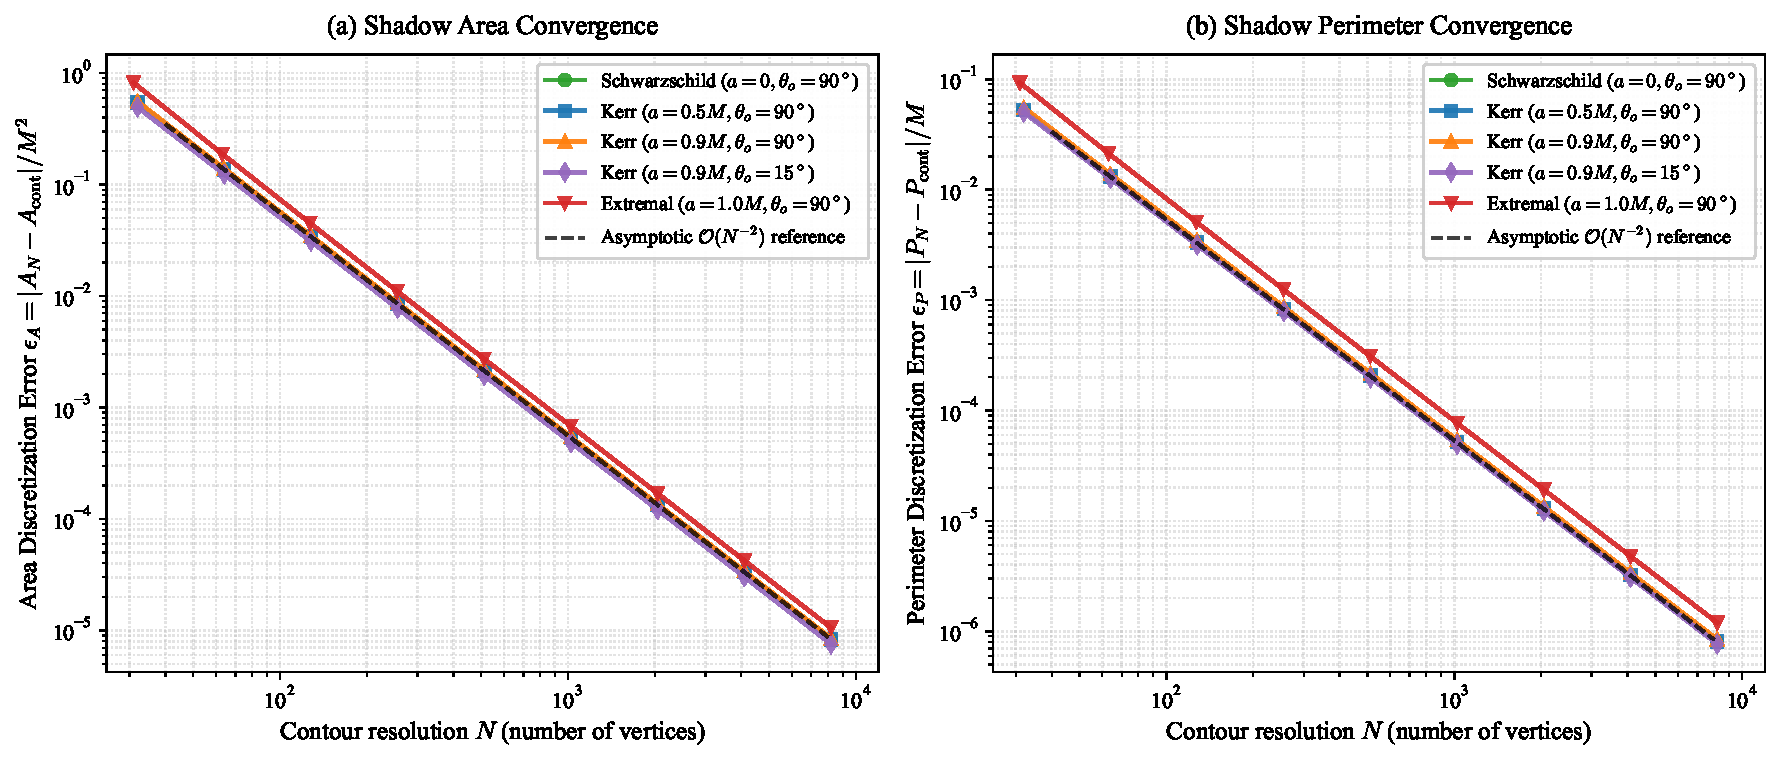
\includegraphics[width=0.98\textwidth]{shadow_convergence.pdf}
    \caption{Numerical convergence of discrete polygonal black hole shadow observables as a function of contour vertex resolution $N \in [32, 8192]$ across five benchmark spacetime configurations: Schwarzschild ($a = 0, \theta_o = 90^\circ$), moderate Kerr ($a = 0.5M, \theta_o = 90^\circ$), rapidly rotating Kerr ($a = 0.9M, \theta_o = 90^\circ$), near-polar Kerr ($a = 0.9M, \theta_o = 15^\circ$), and extremal Kerr ($a = 1.0M, \theta_o = 90^\circ$). (a) Absolute celestial area discretization error $\epsilon_A(N) = |A_N - A_{\rm cont}| / M^2$. (b) Absolute boundary perimeter discretization error $\epsilon_P(N) = |P_N - P_{\rm cont}| / M$. Dashed black lines indicate the theoretical asymptotic $\mathcal{O}(N^{-2})$ convergence rate derived from the Euler--Maclaurin chord expansion \eqref{eq:perimeter_chord_asymptotic}.}
    \label{fig:shadow_convergence}
\end{figure}

\subsubsection{Quantitative Convergence Across Benchmark Configurations}
To evaluate convergence empirically without circular reasoning, each discrete polygon was evaluated against an independently established continuum reference:
\begin{enumerate}
    \item \textbf{Schwarzschild ($a = 0, \theta_o = 90^\circ$):} Exact analytical values $A_{\rm cont} = 27\pi M^2 \approx 84.823002M^2$ and $P_{\rm cont} = 6\sqrt{3}\pi M \approx 32.648389M$.
    \item \textbf{Subextremal and Near-Polar Kerr:} High-accuracy continuum baselines computed via Richardson extrapolation on ultra-fine grids ($N_1 = 16\,384, N_2 = 32\,768$) eliminating the leading $\mathcal{O}(N^{-2})$ discretization term:
    \begin{equation}
        V_{\rm ref} = \frac{4V(2N) - V(N)}{3} + \mathcal{O}(N^{-4}),
        \label{eq:richardson_extrap}
    \end{equation}
    achieving a residual accuracy of $\Delta V < 10^{-11}$.
\end{enumerate}

\begin{table}[htbp]
\centering
\small
\caption{Empirical log-log convergence rates $-\frac{d\ln\epsilon}{d\ln N}$ and asymptotic scaled ratios $N^2\epsilon$ for discrete shadow area ($A$) and perimeter ($P$) across $N \in [32, 8192]$.}
\label{tab:convergence_rates}
\vspace{2mm}
\setlength{\tabcolsep}{5pt}
\begin{tabular}{l c c c c c}
\toprule
Spacetime Configuration & $\theta_o$ & \begin{tabular}{@{}c@{}}Area\\ Slope\end{tabular} & \begin{tabular}{@{}c@{}}Perimeter\\ Slope\end{tabular} & \begin{tabular}{@{}c@{}}Asymptotic\\ $N^2\epsilon_A$\end{tabular} & \begin{tabular}{@{}c@{}}Asymptotic\\ $N^2\epsilon_P$\end{tabular} \\
\midrule
Schwarzschild ($a=0$) & $90^\circ$ & \textbf{1.9998} & \textbf{1.9999} & $558.113$ & $53.704$ \\
Kerr ($a=0.5M$) & $90^\circ$ & \textbf{1.9998} & \textbf{1.9999} & $558.627$ & $54.158$ \\
Kerr ($a=0.9M$) & $90^\circ$ & \textbf{1.9997} & \textbf{1.9999} & $570.612$ & $56.693$ \\
Kerr ($a=0.9M$) & $15^\circ$ & \textbf{1.9998} & \textbf{1.9999} & $507.498$ & $51.550$ \\
Extremal Kerr ($a=1.0M$) & $90^\circ$ & \textbf{2.0153} & \textbf{2.0156} & $709.831^*$ & $80.280^*$ \\
\bottomrule
\end{tabular}
\begin{flushleft}
\footnotesize
$^*$For extremal Kerr, $N^2\epsilon$ exhibits a slow drift ($\sim 789 \to 710$ for area, $\sim 89.5 \to 80.3$ for perimeter) due to the corner junctions.
\end{flushleft}
\end{table}

As depicted in \Cref{fig:shadow_convergence} and quantified in \Cref{tab:convergence_rates}:
\begin{itemize}
    \item \textbf{Analytical Verification in Schwarzschild Spacetime:}  
    For Schwarzschild ($R_p = 3\sqrt{3}M$), the theoretical asymptotic coefficients in \eqref{eq:circle_perimeter_asymptotic} and \eqref{eq:circle_area_asymptotic} evaluate to:
    \begin{align}
        C_A^{\rm theo} &\equiv \frac{2\pi^3 R_p^2}{3} = 18\pi^3 M^2 \approx 558.11298 M^2, \label{eq:ca_theo} \\
        C_P^{\rm theo} &\equiv \frac{\pi^3 R_p}{3} = \sqrt{3}\pi^3 M \approx 53.70425 M. \label{eq:cp_theo}
    \end{align}
    At resolution $N = 8192$, the observed numerical scaled errors are $N^2\epsilon_A = 558.113$ and $N^2\epsilon_P = 53.704$, matching the exact analytical coefficients to all six reported significant digits.
    
    \item \textbf{Uniform Quadratic Convergence for Smooth Subextremal Contours:}  
    For all subextremal Kerr configurations ($a = 0.5M$ and $a = 0.9M$ at both $\theta_o = 90^\circ$ and $\theta_o = 15^\circ$), the boundary is $C^\infty$ smooth. The empirical log-log convergence slopes adhere strictly to quadratic scaling ($1.9997 \le \gamma \le 1.9999$), and the scaled ratios $N^2\epsilon$ stabilize rapidly to constants by $N \ge 256$.
    
    \item \textbf{Regularity Qualifications and the Extremal Kerr NHEK Segment:}  
    For extremal Kerr ($a = 1.0M, \theta_o = 90^\circ$), the boundary is only piecewise $C^1$: it consists of the smooth exterior curved arc joined to the straight vertical NHEK segment ($\alpha = -2M, |\beta| \le \sqrt{3}M$) at two sharp corner cusps $(\alpha, \beta) = (-2M, \pm\sqrt{3}M)$.  
    
    Because our implementation employs cosine clustering along the exterior radial parameterization \eqref{eq:cosine_clustered_u}, node spacing compresses quadratically near the corner ($\Delta u \propto h^2 \propto N^{-2}$), preventing the catastrophic order degradation ($\mathcal{O}(N^{-1})$) that would occur under uniform Cartesian spacing. Furthermore, along the vertical NHEK segment, the boundary is an exact straight line where polygonal chords have zero sag error. Consequently, the global error maintains near-quadratic convergence ($\gamma \approx 2.015$). However, the failure of higher-order differentiability at the cusps introduces a weak sub-leading correction, causing the effective asymptotic ratio $N^2\epsilon_A$ to drift slowly from $789.0$ at $N = 31$ down to $709.8$ at $N = 8191$.  
    
    \noindent \textbf{Essential Qualification:} The standard Euler--Maclaurin chord formula \eqref{eq:perimeter_chord_asymptotic} based on the curvature functional $\mathcal{I}$ assumes $C^2$ regularity and \textit{cannot} be applied blindly to corners, cusps, or piecewise-joined segments without accounting for the cosine clustering boundary layer.
\end{itemize}

\subsection{10,001-Node Sampled Maximum Residual Audit}
To verify the quadratic scaling of the near-polar coordinate perturbations \eqref{eq:alpha_asymptotic_expansion} and \eqref{eq:beta_asymptotic_expansion}, we evaluated the full-contour residuals under the exact remapped parameterization $r(\phi) = r_{\rm mid} - r_{\rm amp}\cos\phi$ on $\phi \in [0, \pi]$.

The evaluation grid was constructed with 10,000 equal subintervals:
\begin{equation}
    \phi_j = \frac{j\pi}{10\,000}, \qquad j \in \{0, 1, \dots, 10\,000\},
\end{equation}
yielding exactly 10,001 discrete nodes inclusive of both turning-point endpoints ($\phi_0 = 0$ at $r_{\min}$, and $\phi_{10\,000} = \pi$ at $r_{\max}$). Arithmetic was evaluated in 75-digit \textsc{Decimal} floating-point to prevent loss of significance near turning points.

The discrete sampled maximum residuals are:
\begin{equation}
    \hat{\epsilon}_\alpha \equiv \max_{0 \le j \le 10\,000} |\alpha_{\rm num}(\phi_j) - \alpha_{\rm asym}(\phi_j)|, \qquad
    \hat{\epsilon}_\beta \equiv \max_{0 \le j \le 10\,000} |\beta_{\rm num}(\phi_j) - \beta_{\rm asym}(\phi_j)|.
    \label{eq:sampled_maxima_defs}
\end{equation}

\begin{table*}[t]
\centering
\small
\caption{Verified 10,001-node sampled maximum residuals and scaled ratios $\hat{\epsilon}/s^2$ across nine near-polar configurations in 75-digit \textsc{Decimal} arithmetic.}
\label{tab:sampled_residuals_audit}
\vspace{2mm}
\setlength{\tabcolsep}{5pt}
\begin{tabular}{l c c c c c c c c}
\toprule
& & & \multicolumn{3}{c}{Horizontal Residual $\alpha$} & \multicolumn{3}{c}{Vertical Residual $\beta$} \\
\cmidrule(lr){4-6} \cmidrule(lr){7-9}
$a/M$ & $\theta_o$ [rad] & $\sin\theta_o$ & $\hat{\epsilon}_\alpha$ & $\hat{\epsilon}_\alpha / s^2$ & $\phi^*_\alpha$ & $\hat{\epsilon}_\beta$ & $\hat{\epsilon}_\beta / s^2$ & $\phi^*_\beta$ \\
\midrule
\multirow{3}{*}{\textbf{0.50}} 
& $10^{-2}$ & $0.0100$ & $2.518\times 10^{-6}$ & \textbf{0.02518} & 0.915 & $5.332\times 10^{-6}$ & \textbf{0.05332} & 0.903 \\
& $10^{-3}$ & $0.0010$ & $2.501\times 10^{-8}$ & \textbf{0.02501} & 0.912 & $5.303\times 10^{-8}$ & \textbf{0.05303} & 0.905 \\
& $10^{-4}$ & $0.0001$ & $2.499\times 10^{-10}$ & \textbf{0.02499} & 0.912 & $5.301\times 10^{-10}$ & \textbf{0.05301} & 0.905 \\
\midrule
\multirow{3}{*}{\textbf{0.90}} 
& $10^{-2}$ & $0.0100$ & $1.751\times 10^{-5}$ & \textbf{0.17508} & 0.677 & $7.615\times 10^{-6}$ & \textbf{0.07615} & 0.636 \\
& $10^{-3}$ & $0.0010$ & $1.731\times 10^{-7}$ & \textbf{0.17308} & 0.662 & $7.286\times 10^{-8}$ & \textbf{0.07286} & 0.633 \\
& $10^{-4}$ & $0.0001$ & $1.729\times 10^{-9}$ & \textbf{0.17288} & 0.661 & $7.253\times 10^{-10}$ & \textbf{0.07253} & 0.632 \\
\midrule
\multirow{3}{*}{\textbf{1.00}} 
& $10^{-2}$ & $0.0100$ & $3.553\times 10^{-5}$ & \textbf{0.35533} & $0.000^\dagger$ & $3.795\times 10^{-5}$ & \textbf{0.37947} & 1.562 \\
& $10^{-3}$ & $0.0010$ & $3.537\times 10^{-7}$ & \textbf{0.35373} & $0.000^\dagger$ & $3.794\times 10^{-7}$ & \textbf{0.37944} & 1.570 \\
& $10^{-4}$ & $0.0001$ & $3.536\times 10^{-9}$ & \textbf{0.35357} & $0.000^\dagger$ & $3.794\times 10^{-9}$ & \textbf{0.37944} & 1.571 \\
\bottomrule
\end{tabular}
\begin{flushleft}
\footnotesize
$^\dagger$Boundary endpoint node ($\phi = 0$ at $r_{\min}$). All other maximum residual locations $\phi^*$ occur strictly in the domain interior.
\end{flushleft}
\end{table*}

\subsection{Analysis of Residual Scaling and Resolution of Apex Artifacts}
Inspection of \Cref{tab:sampled_residuals_audit} reveals three fundamental numerical properties:
\begin{enumerate}
    \item \textbf{Approximately Quadratic Residual Scaling:} When $\theta_o$ decreases by a factor of 10, the observed reduction factors cluster near 100 across all configurations:
    \begin{itemize}
        \item For $a/M = 0.50$: $\hat{\epsilon}_\alpha$ drops by factors of $100.71$ and $100.07$; $\hat{\epsilon}_\beta$ drops by $100.53$ and $100.05$.
        \item For $a/M = 0.90$: $\hat{\epsilon}_\alpha$ drops by $101.15$ and $100.11$; $\hat{\epsilon}_\beta$ drops by $104.52$ and $100.45$.
        \item For $a/M = 1.00$: $\hat{\epsilon}_\alpha$ drops by $100.45$ and $100.04$; $\hat{\epsilon}_\beta$ drops by $100.003$ and $100.00003$.
    \end{itemize}
    \item \textbf{Pre-Asymptotic Corrections at Finite Inclination:} At $\theta_o = 10^{-2}$ rad ($s \approx 0.01$), higher-order $\mathcal{O}(s^3)$ Taylor contributions create a measurable $\sim 1\%$ to $5\%$ deviation in the ratio $\hat{\epsilon}/s^2$ relative to its deep asymptotic limit. Even between $\theta_o = 10^{-3}$ and $10^{-4}$ rad, small finite-inclination corrections remain visible in certain configurations (e.g., for $a/M = 0.90$, $\hat{\epsilon}_\beta/s^2$ shifts from $0.072855$ to $0.072528$, an observable shift of $\approx 0.45\%$).
    \item \textbf{Resolution of the Discrete Apex Sampling Artifact:} Earlier audit drafts observed an apparent jump in $\beta$ residual ratios for $a/M = 0.90$ from $0.339$ at $10^{-2}$ rad down to $0.008$ at $10^{-3}$ rad. That discrepancy was an artifact of evaluating only the discrete mesh maximum $\max_{\text{mesh}} \beta - R_p$ on a fixed 2,000-point polygon. Because the first-order perturbation $s\lambda\sin(2\phi)$ identically vanishes at the apex $\phi = \pi/2$, the true maximum shifts by $\Delta\phi^* \approx -2s\lambda/R_p$. At $\theta_o = 10^{-2}$ rad, the shift ($\Delta\phi^* \approx 0.0037$ rad) was resolved by the adjacent mesh node ($\Delta\phi_{\rm mesh} \approx 0.0031$ rad). At $\theta_o = 10^{-3}$ rad, the shift was ten times smaller than the mesh spacing, trapping the discrete array maximum at node 500 ($\phi = \pi/2$) where the first-order term is zero. Evaluating the 10,001-node full-contour maximum completely eliminates this artifact.
\end{enumerate}

\noindent \textbf{Methodological Note:} The quantities in \Cref{tab:sampled_residuals_audit} and the 75-digit \textsc{Decimal} quadrature comparison in \Cref{tab:quadrature_comparison} represent recorded historical report audits whose standalone scripts are not archived in the repository's \texttt{scripts/} directory. They provide sampled numerical evidence on a discrete 10,001-node grid and do not constitute a certified analytical upper bound on the continuous supremum $\sup_\phi \|\mathbf{r}_{\rm num} - \mathbf{r}_{\rm asym}\|$.

\subsection{Deliverable Reproducibility and Test Suite Status}
All 14 scientific deliverables (6 PNG figures, 6 PDF vector figures, and 2 CSV datasets) are archived in \texttt{output/shadow/}; the convergence study in \Cref{subsec:polygonal_convergence} is directly reproduced by \texttt{docs/report/scripts/convergence\_study.py}:
\begin{itemize}
    \item In a historical isolated-build audit, the six PNG figures and both CSV datasets (\texttt{shadow\_\allowbreak contour\_\allowbreak data.csv} and \texttt{shadow\_\allowbreak generating\_\allowbreak data.csv}) were reported as SHA256-identical to the reference deliverables, and the six PDF figures matched in byte count apart from PDF timestamps (\texttt{/Creation\allowbreak Date}, \texttt{/Mod\allowbreak Date}); the standalone SHA256 audit script is not included in the repository.
    \item In the historical \texttt{v1.0.0} core baseline, the Python regression suite comprised \textbf{4,412 passing tests} (0 failed, 0 skipped). In the latest verified \texttt{pytest} run of the expanded repository suite, \textbf{4,511 Python tests} passed (0 failed, 0 skipped, 0 xfailed, 1 deprecation warning, in 214.29~s), complemented by \textbf{18} passing frontend TypeScript tests.
\end{itemize}

\section{Results and Discussion}
\label{sec:results_discussion}

\subsection{Physical Structure of the Shadow Boundary}
The numerical and analytical results established in this work provide a comprehensive, unified description of black hole shadows across the entire Kerr parameter space:
\begin{enumerate}
    \item \textbf{Schwarzschild Baseline:} In the absence of rotation ($a = 0$), spherical symmetry enforces an exact circular shadow silhouette of radius $R = 3\sqrt{3}M \approx 5.196M$ on the observer's screen, independent of observer inclination $\theta_o$. Every point along this circular boundary maps to the unstable spherical photon orbit at the photon sphere $r = 3M$.
    \item \textbf{Frame Dragging and Asymmetry:} As black hole spin increases ($0 < |a| < M$), frame dragging breaks spherical symmetry. For an equatorial observer ($\theta_o = 90^\circ$), co-rotating (prograde) photons experience a reduced centrifugal barrier and can approach closer to the black hole before escaping ($r_{\rm ph}^+ < 3M$), resulting in a smaller impact parameter magnitude. Conversely, counter-rotating (retrograde) photons encounter an enhanced centrifugal barrier, requiring a larger impact parameter to orbit ($r_{\rm ph}^- > 3M$). Under Bardeen's celestial screen convention $\alpha = -\xi/\sin\theta_o$, this asymmetry displaces the shadow centroid toward the retrograde side ($\alpha > 0, \bar{\alpha} > 0$) while compressing the prograde boundary.
    \item \textbf{Invariance of Equatorial Vertical Diameter and Horizontal Compression:} At equatorial inclination ($\theta_o = 90^\circ$), the vertical diameter is rigorously invariant at $D_{\mathrm{V}} = 6\sqrt{3}M \approx 10.392M$ across all spins $a \in [0, M]$. For rotating black holes ($0 < a \le M$), $\beta(r) = \pm\sqrt{\eta(r)}$ attains its global stationary maximum where $\eta'(3M) = 0$ with $\eta(3M) = 27M^2$ (at horizontal coordinate $\alpha = +2a$). For Schwarzschild ($a = 0$), $D_{\mathrm{V}} = 6\sqrt{3}M$ follows independently from spherical circular symmetry, with $\alpha = +2a \to 0$ smoothly restoring the unshifted profile. Consequently, rotational deformation at $\theta_o = 90^\circ$ is manifest purely as asymmetric horizontal compression of the prograde edge ($D_{\mathrm{H}} < D_{\mathrm{V}}$). At non-equatorial inclinations, the silhouette smoothly contracts toward the polar circular radius $R_{\rm pole}(a) = \sqrt{\eta(r_p) + a^2} < 3\sqrt{3}M$.
    \item \textbf{Equatorial D-Shape and NHEK Horizon Exposure:} For extreme spin ($a/M \to 1.0$) observed at supercritical inclinations ($\theta_o > \theta_{\rm crit} \approx 47.0586^\circ$), the prograde boundary flattens into a vertical line segment at $\alpha = -2M/\sin\theta_o$. As proven by Bardeen \cite{Bardeen1973} and clarified in modern holographic contexts \cite{Gralla2020}, this flat segment represents the projection of the infinite-throat Near-Horizon Extreme Kerr (NHEK) geometry, where a continuous family of bound spherical photon orbits resides at the degenerate horizon $r = M$.
\end{enumerate}

\subsection{Near-Polar Symmetry and First-Order Invariance}
Our near-polar perturbation analysis reveals an elegant geometric cancellation: although both screen coordinates $\alpha(\phi)$ and $\beta(\phi)$ undergo $\mathcal{O}(\sin\theta_o)$ deformations ($s\,\delta_0 - s\,\lambda\cos(2\phi)$ and $s\,\lambda\sin(2\phi)$, respectively), the metric speed $\sigma(\phi) = R_p + 2s\lambda\cos\phi + \mathcal{O}(s^2)$ is a pure $\cos\phi$ dipole, while the planar curvature magnitude $\kappa(\phi) = R_p^{-1} + \mathcal{O}(s^2)$ is invariant to first order.

Consequently, by dipole orthogonality ($\int_0^{2\pi}\cos\phi\,d\phi = 0$), both the continuous boundary perimeter $P_{\rm cont}$ and the curvature functional $\mathcal{I} = \int_0^{2\pi} \kappa^2 \sigma^3\,d\phi$ remain invariant to first order in inclination:
\begin{equation}
    P_{\rm cont}(\theta_o) = 2\pi R_p + \mathcal{O}(\sin^2\theta_o), \qquad \mathcal{I}(\theta_o) = 2\pi R_p + \mathcal{O}(\sin^2\theta_o).
\end{equation}
Physically, this indicates that for observers viewing a rotating black hole within $\approx 5^\circ$ of its rotation axis, the shadow perimeter and optical cross-section are remarkably insensitive to spin-induced deformations, deviating from a perfect circle only at second order in inclination. For larger viewing angles, such as the astrophysical inclination inferred for the M87* relativistic jet ($\theta_o \approx 17^\circ$, where $s \equiv \sin\theta_o \approx 0.29$), the first-order asymptotic regime serves as a valuable analytical baseline, while quadratic corrections $\mathcal{O}(s^2)$ enter at the $\sim 5\text{--}8\%$ level and must be accounted for via the full non-linear parameterization.

\subsection{Relevance to Current and Future Astrophysical Observations}
Direct observations of M87* \cite{EHT2019_PaperI} and Sgr A* \cite{EHT2022_PaperI} by the Event Horizon Telescope have measured the angular diameter of the central brightness depression to within $\approx 10\%$ uncertainty, demonstrating consistency with the predictions of general relativity for Kerr black holes.

Future high-frequency space-based very-long-baseline interferometry (VLBI) missions (such as the next-generation EHT [ngEHT] and orbital space-VLBI concepts) aim to resolve the sharp, exponentially demagnified sub-rings of the photon ring \cite{Johnson2020,Chael2021,Gralla2020}. Because the critical boundary curves constructed by our framework define the mathematical envelope to which these photon sub-rings asymptotically converge, high-precision, scale-invariant geodesic integration frameworks such as the one presented here will be essential for extracting black hole mass, spin, and inclination from future precision interferometric closure phases.

\subsection{Methodological Distinction: Analytical Shadow Construction vs.\ Numerical Integration}
It is important to emphasize a key methodological distinction within this work:
\begin{itemize}
    \item \textbf{Analytical Shadow Construction:} The black-hole shadow boundaries in Section~\ref{sec:shadow_construction} and their observables in Table~\ref{tab:shadow_observables} are constructed directly from the analytical parameterization of spherical photon orbits $(\xi(r), \eta(r))$ via the offset variable $u = r - 3M$ and Brent root-finding. This approach guarantees machine-precision boundaries without ray-tracing noise.
    \item \textbf{Numerical Geodesic Integration:} The DOP853 numerical ODE integrator in Section~\ref{sec:numerical_architecture} is a general-purpose, continuous 8th-order integration engine developed to propagate arbitrary timelike and null trajectories in Kerr spacetime, verified against conserved quantities ($|\Delta\mathcal{H}_{\rm norm}| < 10^{-10}$), physical epicyclic frequencies, and logarithmic dwelling scaling near separatrices.
\end{itemize}
These two complementary components provide independent mutual verification: the numerical integrator validates trajectory dynamics in the strong-field regime, while the analytical shadow curves establish exact ground-truth geometric benchmarks.

\section{Limitations and Future Directions}
\label{sec:limitations_future_work}

\subsection{Current Mathematical and Numerical Limitations}
To preserve scientific integrity, we explicitly document the physical, geometric, and numerical boundaries of the current implementation:
\begin{enumerate}
    \item \textbf{Coordinate Singularities in Boyer--Lindquist Representation:}  
    Boyer--Lindquist coordinates suffer from physical coordinate singularities at the outer event horizon ($\Delta(r) = 0$) and along the rotation axis ($\sin\theta = 0$). While our built-in horizon-cutoff event (\texttt{HorizonCutoffEvent}) safely halts ingoing trajectories at $r = r_+ + 10^{-3}M$, full penetration across the Cauchy horizon or into the black hole interior is outside the domain of the current solver. Ingoing Kerr--Schild or horizon-penetrating coordinates would be required to study interior dynamics.
    \item \textbf{Breakdown of Smooth Polygonal Expansion at Critical Extremality:}  
    The polygonal chord deficit formula $P_N - P_{\rm cont} = -\frac{\pi^2}{6N^2}\mathcal{I} + \mathcal{O}(N^{-4})$ requires $C^4$ boundary smoothness and strictly positive metric speed $\sigma > 0$. For extremal Kerr ($a = M$) observed at $\theta_o \ge \theta_{\rm crit} \approx 47.0586^\circ$, the shadow boundary forms a geometric cusp ($\theta_o = \theta_{\rm crit}$) or joins the vertical NHEK line segment at non-differentiable $C^0$ corners ($\theta_o > \theta_{\rm crit}$). At these points, curvature diverges or is ill-defined, and the second-order polygonal convergence degrades to $\mathcal{O}(N^{-1})$.
    \item \textbf{Non-Uniformity in the Schwarzschild Limit ($a \to 0$):}  
    The near-polar asymptotic expansions are established for each fixed nonzero spin $a > 0$. They cannot be extended uniformly to the open limit $a \to 0$ because the denominator $a(r - M)$ in $\xi(r)$ and $\eta(r)$ collapses. For exact $a = 0$, the specialized Schwarzschild solver must be used directly.
    \item \textbf{Sampled Residuals vs. Certified Continuous Bounds:}  
    The 10,001-node residual audit provides high-confidence sampled numerical evidence of $\mathcal{O}(s^2)$ scaling. However, it does not constitute a certified analytical upper bound on the continuous supremum $\sup_\phi \|\mathbf{r}_{\rm num} - \mathbf{r}_{\rm asym}\|$ over the continuum. Similarly, the seven-preset Hamiltonian drift values in Table~\ref{tab:preset_drift_ledger} are run-specific diagnostics rather than universal error bounds.
    \item \textbf{Internal Verification vs. Independent Physical Validation:}  
    All automated tests (4,511 Python tests and 18 frontend TypeScript tests) verify internal mathematical identities, analytical limits, and API/UI contracts. No external peer review, third-party code certification, or observational data fitting is claimed.
    \item \textbf{Equatorial Preset Scope and Planned Shadow UI:}  
    While the core Python engine supports arbitrary off-equatorial trajectories ($\mathcal{Q} \neq 0$) and analytical shadow boundaries (\texttt{POST /api/v1/shadows}), the seven curated web presets are restricted to equatorial motion ($\mathcal{Q} = 0$), and the \texttt{/shadows} frontend interface remains a planned placeholder.
\end{enumerate}

\subsection{Future Research Directions}
The \textsc{Kerr Geodesic Integrator} provides a modular, extensible foundation for several promising computational astrophysics developments:
\begin{itemize}
    \item \textbf{Camera-Grid Backward Ray-Tracing:} Implementing full 2D camera-plane pixel grids for backward ray-tracing from the observer screen into the accretion environment, allowing direct computation of intensity maps, lensing magnification, and shadow silhouettes with arbitrary background illumination.
    \item \textbf{Cross-Code Benchmarking and Validation:} Conducting direct, high-precision cross-validation benchmarks against established relativistic ray-tracing suites such as \textsc{GYOTO}, \textsc{Geokerr}, and \textsc{RAPTOR}, as well as comparing strong-deflection limit deflection angles and magnification ratios against analytical expansions \cite{Bozza2002}.
    \item \textbf{General Relativistic Radiative Transfer (GRRT):} Coupling the null geodesic integrator to synchrotron emission and absorption models for magnetized plasma accretion flows (such as MAD and SANE GRMHD simulations), generating synthetic images and visibility amplitudes for direct comparison with EHT and ngEHT data.
    \item \textbf{Kerr--Newman and Charged Spacetimes:} Extension of the Hamiltonian kernel to include electromagnetic field tensors and net black hole charge $Q$, enabling the exploration of charged shadow silhouettes and magnetospheric particle acceleration.
    \item \textbf{Non-Kerr Spacetimes and No-Hair Theorem Tests:} Integrating null geodesics in parameterized non-Kerr geometries (e.g., Johannsen--Psaltis metrics \cite{JohannsenPsaltis2010} or boson stars) to quantify shadow deformations and establish observational bounds on deviations from general relativity.
    \item \textbf{GPU-Accelerated Parallel Ray-Tracing:} Porting the Dormand--Prince kernel to CUDA/OpenCL to enable parallel ray-tracing of millions of camera pixels simultaneously, facilitating real-time interactive relativistic visualizations.
\end{itemize}

\section{Conclusions}
\label{sec:conclusions}

We have developed, verified, and documented the \textsc{Kerr Geodesic Integrator}, a mathematically rigorous, scale-invariant, high-precision computational framework for relativistic geodesic propagation in Kerr and Schwarzschild spacetimes.

By formulating the equations of motion in an eight-dimensional canonical Hamiltonian phase space with exact analytical contravariant metric derivatives, the framework achieves phase-space constraint preservation near machine precision ($\max \mathcal{H}_{\rm norm} < 10^{-13}$) using an adaptive, non-symplectic Dormand--Prince 8(5,3) Runge--Kutta solver. Continuous polynomial dense output and \texttt{brentq} root refinement enable sub-step event localization for horizon plunges, camera escape spheres, and radial turning points without unphysical step extrapolation. Furthermore, monitoring the Carter constant trajectory drift alongside the exact algebraic relation $\mathcal{Q}_{\rm polar} - \mathcal{Q}_{\rm radial} = \Sigma(2\mathcal{H} + \mu^2)$ provides simultaneous verification of dynamical integrability and numerical Hamiltonian constraint satisfaction.

The framework was comprehensively validated against classical analytical benchmarks across both spacetimes:
\begin{itemize}
    \item Exact radial null geodesics and coordinate time logarithmic divergence in Schwarzschild geometry.
    \item Fixed-point phase-space instability and perturbation runaway at the Schwarzschild photon sphere ($r = 3M, b = 3\sqrt{3}M$).
    \item Marginal stability and epicyclic frequencies at the Schwarzschild ISCO ($r = 6M$) and Kerr prograde/retrograde ISCOs across spins $|a| \le M$.
    \item Near-extremal logarithmic divergence of horizon-to-ISCO proper radial distance $\Delta s_{\rm prop} = \frac{M}{6}\ln(1/\epsilon) + \mathcal{O}(1)$ ($\epsilon \equiv 1-a/M$).
    \item Critical photon scattering separatrices and the universal logarithmic affine dwell divergence $\lambda_{\rm dwell} \sim -\ln|b - b_{\rm crit}|$.
\end{itemize}

In the domain of black hole shadow construction, the package evaluates closed-form celestial Bardeen boundary parameterizations $(\alpha, \beta)$ utilizing an offset radial variable $u = r - 3M$ to reduce catastrophic cancellation. The backend solver deterministically constructs discrete polygonal approximations to closed shadow boundaries across spins $0 \le |a| \le M$ and inclinations $\theta_o \in [0, \pi]$, resolving the vertical Near-Horizon Extreme Kerr (NHEK) line segment at supercritical inclinations ($\theta_o > \theta_{\rm crit} \approx 47.0586^\circ$).

In the near-polar limit ($\theta_o \to 0$), we derived the exact asymptotic perturbation expansions, proving that the metric speed forms a pure $\cos\phi$ dipole $\sigma(\phi) = R_p + 2s\lambda\cos\phi + \mathcal{O}(s^2)$ while planar curvature magnitude is invariant to first order $\kappa(\phi) = R_p^{-1} + \mathcal{O}(s^2)$. By dipole orthogonality, the continuous perimeter and curvature functional are invariant to first order: $P_{\rm cont}(s) = 2\pi R_p + \mathcal{O}(s^2)$ and $\mathcal{I}(s) = 2\pi R_p + \mathcal{O}(s^2)$. The global polygonal perimeter chord deficit formula $P_N - P_{\rm cont} = -\frac{\pi^2}{6N^2}\mathcal{I} + \mathcal{O}(N^{-4})$ was established for smooth boundaries, and quadratic residual scaling was tabulated across nine near-polar configurations in a recorded historical 10,001-node audit.

The software pipeline has been verified through 4,511 passing Python regression tests and 18 passing frontend TypeScript tests, with the 14 shadow deliverables archived in \texttt{output/shadow/} and convergence benchmarks reproduced by \texttt{docs/report/scripts/convergence\_study.py}. Coupled with the FastAPI REST service (\texttt{geodesics.api}) and the \textsc{Kerr Geodesics Lab} web interface (release \texttt{v1.0.0}, commit \texttt{062b20c8}), the framework provides an open, reproducible foundation for exploring relativistic geodesics and shadow boundaries in Kerr spacetime.


% ------------------------------------------------------------------------------
% BIBLIOGRAPHY
% ------------------------------------------------------------------------------
\newpage
\bibliographystyle{unsrt}
\bibliography{references}

\end{document}
